%
% Niniejszy plik stanowi przykład formatowania pracy magisterskiej na
% Wydziale MIM UW.  Szkielet użytych poleceń można wykorzystywać do
% woli, np. formatujac wlasna prace.
%
% Zawartosc merytoryczna stanowi oryginalnosiagniecie
% naukowosciowe Marcina Wolinskiego.  Wszelkie prawa zastrzeżone.
%
% Copyright (c) 2001 by Marcin Woliński <M.Wolinski@gust.org.pl>
% Poprawki spowodowane zmianami przepisów - Marcin Szczuka, 1.10.2004
% Poprawki spowodowane zmianami przepisow i ujednolicenie 
% - Seweryn Karłowicz, 05.05.2006
% Dodanie wielu autorów i tłumaczenia na angielski - Kuba Pochrybniak, 29.11.2016

% dodaj opcję [licencjacka] dla pracy licencjackiej
% dodaj opcję [en] dla wersji angielskiej (mogą być obie: [licencjacka,en])
\documentclass[magisterska]{pracamgr}


% Dane magistranta:
\autor{Mateusz Kiebała}{359758}

\title{Biblioteka do implementacji algorytmów minimalnych}
%\tytulang{A library for implementing minimal algoritms}

%kierunek: 
\kierunek{informatyka}

% informatyka - nie okreslamy zakresu (opcja zakomentowana)
% matematyka - zakres moze pozostac nieokreslony,
% a jesli ma byc okreslony dla pracy mgr,
% to przyjmuje jedna z wartosci:
% {metod matematycznych w finansach}
% {metod matematycznych w ubezpieczeniach}
% {matematyki stosowanej}
% {nauczania matematyki}
% Dla pracy licencjackiej mamy natomiast
% mozliwosc wpisania takiej wartosci zakresu:
% {Jednoczesnych Studiow Ekonomiczno--Matematycznych}

% \zakres{Tu wpisac, jesli trzeba, jedna z opcji podanych wyzej}

% Praca wykonana pod kierunkiem:
% (podać tytuł/stopień imię i nazwisko opiekuna
% Instytut
% ew. Wydział ew. Uczelnia (jeżeli nie MIM UW))
\opiekun{dr Jacka Sroki}

% miesiąc i~rok:
\date{Październik 2019}

%Podać dziedzinę wg klasyfikacji Socrates-Erasmus:
\dziedzina{ 
%11.0 Matematyka, Informatyka:\\ 
%11.1 Matematyka\\ 
%11.2 Statystyka\\ 
11.3 Informatyka\\
%11.4 Sztuczna inteligencja\\ 
%11.5 Nauki aktuarialne\\
%11.9 Inne nauki matematyczne i informatyczne
}

%Klasyfikacja tematyczna wedlug AMS (matematyka) lub ACM (informatyka)
\klasyfikacja{
Software and its engineering -- Software notations and tools \\
Software and its engineering -- Cloud computing \\
Software and its engineering -- Frameworks \\
Theory of computation — Design and analysis of algorithms \\
Theory of computation -- MapReduce algorithms \\
Computer systems organization -- Cloud computing \\
}

% Słowa kluczowe:
\keywords{Spark, Hadoop, MapReduce, algorytmy minimalne, algorytmy rozproszone, programowanie rozproszone, TeraSort, big data}

% Tu jest dobre miejsce na Twoje własne makra i~środowiska:
\newtheorem{defi}{Definicja}[section]
\usepackage{graphicx}
\usepackage{tabularx,ragged2e,booktabs,caption}
\usepackage{algpseudocode}
\usepackage{amsmath}
\usepackage{float}
\usepackage{listings}
\usepackage{xcolor}

\widowpenalty10000
\clubpenalty10000
\colorlet{punct}{red!60!black}
\definecolor{background}{HTML}{EEEEEE}
\definecolor{delim}{RGB}{20,105,176}
\colorlet{numb}{magenta!60!black}
\setcounter{secnumdepth}{3}
\setcounter{tocdepth}{3}

\lstdefinelanguage{json}{
    basicstyle=\normalfont\ttfamily,
    numbers=left,
    numberstyle=\scriptsize,
    stepnumber=1,
    numbersep=8pt,
    showstringspaces=false,
    breaklines=true,
    frame=lines,
    backgroundcolor=\color{background},
    literate=
     *{0}{{{\color{numb}0}}}{1}
      {1}{{{\color{numb}1}}}{1}
      {2}{{{\color{numb}2}}}{1}
      {3}{{{\color{numb}3}}}{1}
      {4}{{{\color{numb}4}}}{1}
      {5}{{{\color{numb}5}}}{1}
      {6}{{{\color{numb}6}}}{1}
      {7}{{{\color{numb}7}}}{1}
      {8}{{{\color{numb}8}}}{1}
      {9}{{{\color{numb}9}}}{1}
      {:}{{{\color{punct}{:}}}}{1}
      {,}{{{\color{punct}{,}}}}{1}
      {\{}{{{\color{delim}{\{}}}}{1}
      {\}}{{{\color{delim}{\}}}}}{1}
      {[}{{{\color{delim}{[}}}}{1}
      {]}{{{\color{delim}{]}}}}{1},
}

\lstdefinelanguage{Java}{
    basicstyle=\normalfont\ttfamily,
    numbers=left,
    numberstyle=\scriptsize,
    stepnumber=1,
    numbersep=8pt,
    showstringspaces=false,
    breaklines=true,
    frame=lines,
    backgroundcolor=\color{background},
    literate=
     *{0}{{{\color{numb}0}}}{1}
      {1}{{{\color{numb}1}}}{1}
      {2}{{{\color{numb}2}}}{1}
      {3}{{{\color{numb}3}}}{1}
      {4}{{{\color{numb}4}}}{1}
      {5}{{{\color{numb}5}}}{1}
      {6}{{{\color{numb}6}}}{1}
      {7}{{{\color{numb}7}}}{1}
      {8}{{{\color{numb}8}}}{1}
      {9}{{{\color{numb}9}}}{1}
      {:}{{{\color{punct}{:}}}}{1}
      {,}{{{\color{punct}{,}}}}{1}
      {\{}{{{\color{delim}{\{}}}}{1}
      {\}}{{{\color{delim}{\}}}}}{1}
      {[}{{{\color{delim}{[}}}}{1}
      {]}{{{\color{delim}{]}}}}{1},
}

\lstdefinelanguage{SmallJava}{
    basicstyle=\footnotesize\ttfamily,
    numbers=left,
    numberstyle=\scriptsize,
    stepnumber=1,
    numbersep=8pt,
    showstringspaces=false,
    breaklines=true,
    frame=lines,
    backgroundcolor=\color{background},
    literate=
     *{0}{{{\color{numb}0}}}{1}
      {1}{{{\color{numb}1}}}{1}
      {2}{{{\color{numb}2}}}{1}
      {3}{{{\color{numb}3}}}{1}
      {4}{{{\color{numb}4}}}{1}
      {5}{{{\color{numb}5}}}{1}
      {6}{{{\color{numb}6}}}{1}
      {7}{{{\color{numb}7}}}{1}
      {8}{{{\color{numb}8}}}{1}
      {9}{{{\color{numb}9}}}{1}
      {:}{{{\color{punct}{:}}}}{1}
      {,}{{{\color{punct}{,}}}}{1}
      {\{}{{{\color{delim}{\{}}}}{1}
      {\}}{{{\color{delim}{\}}}}}{1}
      {[}{{{\color{delim}{[}}}}{1}
      {]}{{{\color{delim}{]}}}}{1},
}

\graphicspath{ {./} }

% koniec definicji

\begin{document}

\maketitle

%tu idzie streszczenie na strone poczatkowa
\begin{abstract}
W ramach pracy magisterskiej stworzono bibliotekę umożliwiającą implementowanie rozproszonych algorytmów minimalnych. Wspiera ona dwa główne frameworki służące do pisania programów rozproszonych: Hadoop i Spark. Celem biblioteki jest udostępnienie zwięzłego API umożliwiającego łatwe implementowanie algorytmów minimalnych. W ramach pracy powstały również implementacje przykładowych algorytmów minimalnych takich jak: tworzenie rankingu, statystyki prefiksowe, grupowanie, pół-złączenia (ang. semi-join) oraz statystyka okienkowa (ang. sliding aggregation).
\end{abstract}
\tableofcontents
%\listoffigures
%\listoftables

\chapter{Wprowadzenie}

W obecnych czasach programowanie rozproszone jest prężnie rozwijającą się dziedziną informatyki. Rozwój technologii i nauki doprowadził do gwałtownego wzrostu gromadzonych danych w różnych dziedzinach życia. Rodzi to potrzebę efektywnego przetwarzania ogromnych zbiorów informacji \cite{watson2014tutorial, wu2013data}.

Obecnie dwoma najbardziej popularnymi frameworkami do przetwarzania dużych danych są Hadoop i Spark \cite{da2015survey}. Pierwszy z nich opiera się na paradygmacie MapReduce \cite{white2012hadoop}, natomiast drugi korzysta z rozproszonych kolekcji danych ze zbiorem typowych operatorów do ich przetwarzania \cite{zaharia2010spark}. W obu systemach algorytm rozproszony uruchamiany jest na grupie niezależnych maszyn, komunikujących się za pomocą sieci, zwanych klastrem obliczeniowym.

Algorytm oparty o paradygmat MapReduce wykonuje się w rundach, a każda runda składa się z trzech faz: \textit{map}, \textit{shuffle} i \textit{reduce}. Podczas faz \textit{map} i \textit{reduce} nie występuje komunikacja między maszynami. W trakcie fazy \textit{map} dane zostają wczytane i wstępnie przetworzone. Następnie faza \textit{shuffle} dba o pogrupowanie i prawidłowe rozesłanie wyników fazy \textit{map} na pamięć lokalną poszczególnych maszyn. W fazie końcowej \textit{reduce}, obliczany jest wynik na podstawie pogrupowanych danych z poprzedniej fazy. Algorytm może posiadać wiele rund. Danymi wejściowymi rundy \textit{i+1} jest wynik działania rundy \textit{i}. Dane pomiędzy rundami są wymieniane poprzez HDFS, co jest kosztownym rozwiązaniem. \cite{shvachko2010hadoop, taylor2010overview, white2012hadoop}.

Spark opiera swoje działanie na elastycznych, rozproszonych zestawach danych (ang. \textit{Resilient Distributed Dataset - RDD}). RDD są niezmienialnymi kolekcjami danych trzymanymi w pamięci podręcznej lub na dyskach lokalnych maszyn. Dzięki bogatemu API operowanie na RDD jest bardzo intuicyjne i efektywne. Nowe RDD tworzone są przez transformacje istniejących \cite{zaharia2010spark}.

Projektując algorytmy działające na Hadoopie i Sparku, trzeba zwrócić uwagę na: równoważenie obciążenia maszyn, zużycie pamięci i CPU, ilość wykonywanych operacji odczytu i~zapisu do plików oraz przesył danych między maszynami. Z tego powodu powstała klasa algorytmów minimalnych, czyli wzorzec algorytmu do którego powinniśmy dążyć. Są to algorytmy rozproszone, gwarantujące zrównoważone zużycie pamięci na każdej z maszyn, ograniczony przesył danych między maszynami, zakończenie algorytmu po stałej liczbie rund / transformacji oraz przyspieszenie obliczeń skalujące się liniowo względem liczby maszyn \cite{tao2013minimal}. 

\section{Motywacja}

Motywacją do napisania biblioteki jest fakt, że spora grupa algorytmów minimalnych opisanych w literaturze bazuje na tych samych obliczeniach początkowych, np. na posortowaniu i zrównoważonym podzieleniu danych, a następnie na przesyłaniu między serwerami ograniczonych statystyk. Celem biblioteki jest udostępnienie optymalnej i łatwej w użyciu bazy algorytmów minimalnych, tak aby zwolnić użytkownika od powtarzalnych czynności przy ich implementowaniu i pozwolić mu skupić się na unikatowej części algorytmu.

Biblioteka do implementacji algorytmów minimalnych redukuje ilość pisanego kodu. \linebreak W przypadku Sparka jest niewielka, ze względu na zwięzłość samego frameworka i bogatego API, jednak w Hadoopie jest bardzo widoczna. Głównie przyczyniają się do tego generalizacja faz MapReduce oraz format danych Avro. Sama tylko możliwość posortowania dowolnych obiektów ma ogromne znaczenie w redukcji kodu. Dodatkowo wszystkie fazy MapReduce i~funkcje udostępniane przez API są generyczne. Wystarczy zdefiniować klasę obiektów, a~reszta implementacji pozostaje stała. Zarówno w Sparku jak i w Hadoopie, do porównywania obiektów używane są komparatory, dzięki czemu użytkownik jeszcze mniejszym nakładem czasu i~pracy może testować różne wersje algorytmu.

Ważnym aspektem rozwiązanym przez bibliotekę jest zarządzanie maszynami. Dzięki abstrakcyjnej numeracji maszyn biblioteka umożliwia przesyłanie danych na dowolnie wybrane z nich. Pozwala to na bardziej precyzyjne zarządzanie transferem danych.

Następną zaletą biblioteki jest ułatwienie przesyłania wielu typów obiektów między fazami i rundami MapReduce w Hadoopie oraz między transformacjami RDD na Sparku. Niektóre algorytmy rozproszone, np. \textit{lista rankingowa} \ref{list_rankingowa}, \textit{statystyki prefiksowe} \ref{statystyki_prefiksowe} wymagają przesyłania wielu rodzajów obiektów jednocześnie. Niestety podstawowe wersje Hadoopa i Sparka nie wspierają takiego rozwiązania. 

Biblioteka pozwala także na definiowanie własnych funkcji statystyk łącznych na zbiorze obiektów. Razem z zaimplementowanymi metodami operującymi na statystykach, biblioteka  pozwala na efektywne obliczanie skomplikowanych statystyk oraz testowanie wielu z nich przy jednorazowej implementacji algorytmu.

\chapter{Podstawowe pojęcia}\label{r:pojecia}
\setlength{\parindent}{6.5ex}
\section{Hadoop}
Podrozdział został napisany w oparciu o \cite{shvachko2010hadoop, taylor2010overview, white2012hadoop}. Hadoop jest otwartym frameworkiem, opartym o język Java, pozwalającym na rozproszone przechowywanie i przetwarzanie dużych zbiorów danych. W tym celu wykorzystuje prosty model programistyczny i rozprasza obliczenia na klastry. Został zaprojektowany z myślą łatwego skalowania. Działa doskonale zarówno na jednej jak i tysiącach maszynach. Dynamiczne dodawanie nowych komputerów do klastra jest łatwe i nieinwazyjne dla działającego systemu. Platforma Hadoop wykorzystuje technikę replikacji danych między maszynami, dzięki czemu zapewniony jest spójny i~ciągły dostęp do danych, nawet w momencie awarii któregoś z serwerów. Dodatkowo Hadoop wykrywa i zarządza błędami warstwy aplikacji. Dzięki temu użytkownik nie musi polegać już na niezawodności sprzętu komputerowego. W skład podstawowej wersji Hadoop wchodzą:

\begin{itemize}
    \item Hadoop Distributed File System (HDFS) -- rozproszony systemem plików (patrz punkt \ref{HDFS}),
    \item Hadoop Common -- zbiór bibliotek (patrz punkt \ref{Hadoop Common}),
    \item Hadoop MapReduce -- framework do implementacji aplikacji rozproszonych (patrz punkt \ref{Hadoop MapReduce}),
    \item YARN -- system zarządzania zasobami klastra (patrz punkt \ref{YARN}).
\end{itemize}

Oprócz wymienionych wyżej modułów istnieją także w pełni zintegrowane rozszerzenia, ułatwiające zarządzanie danymi oraz usługami klastra. Poza otwartym rozwiązaniem, które skupiło wokół siebie sporą grupę kontrybutorów, istnieją także dystrybucje komercyjne. Posiadają one dodatkowe narzędzia tworzące gotowy serwis do przetwarzania dużych danych. Dodatkową zaletą takich rozwiązań jest wsparcie całego ekosystemu Hadoop, a nie tylko poszczegónych modułow.

\subsection{Hadoop Distributed File System (HDFS)} \label{HDFS}

HDFS to rozproszony systemem plików, przeznaczony do przechowywania ogromnych zbiorów danych. Wyróżniają go odporność  na awarie serwerów oraz wysoka jakość pracy na niskobudżetowym sprzęcie komputerowym. Obecnie klastry składają się z tysięcy maszyn. Każda z~nich ma niezerowe prawdopodobieństwo zepsucia się. W praktyce oznacza to, że często któraś z maszyn nie działa. Dlatego też, wykrywanie, reagowanie i szybkie naprawianie usterek jest fundamentalną częścią HDFS.

Architektura HDFS składa się z serwera nadzorującego (\textit{NameNode}) oraz maszyn wykonawczych (\textit{DataNodes}). Dane są zapisywane w postaci plików. HDFS jest systemem niezawodnym w kontekście przechowywania danych. Każdy plik jest trzymany jako sekwencja bloków, gdzie wszystkie oprócz ostatniego są tej samej wielkości. Bloki natomiast są replikowane i przechowywane na wielu \textit{DataNodes}. \textit{NameNode} jest odpowiedzialny za otwieranie, zamykanie i nazywanie plików i folderów. Zarządza także mapowaniem bloków plików na \textit{DataNodes}. \textit{DataNodes} są natomiast odpowiedzialne za tworzenie, usuwanie i replikację bloków oraz za obsługiwanie poleceń czytania i pisania do bloków.

\subsection{Hadoop Common} \label{Hadoop Common}

Hadoop Common jest zbiorem bibliotek wspierającym i integrującym pozostałe moduły Hadoopa. Tworzy warstwę abstrakcji do zarządzania systemem oraz dostępem do HDFS. Zawiera także niezbędne pliki JAR oraz skrypty pozwalające na uruchomienie Hadoopa. Dodatkowo udostępnia kod źródłowy oraz dokumentację Hadoopa.

\subsection{Hadoop MapReduce} \label{Hadoop MapReduce}

Hadoop MapReduce jest frameworkiem opartym o paradygmat MapReduce, służącym do łatwego implementowania aplikacji rozproszonych, operujących na ogromnych zbiorach danych. Pozwala na przetwarzanie nieustrukturyzowanych danych, zapewniającym przy tym niezawodność oraz odporność programu na awarie. 

MapReduce operuje wyłącznie na parach \textit{<klucz, wartość>}. Typy \textit{klucz} oraz \textit{wartość} muszą być serializowalne przez framework oraz muszą implementować komparatory. Początkowo główny proces MapReduce dzieli dane wejściowe na niezależne paczki, które są następnie przetwarzane w sposób równoległy przez procesy \textit{map}. Kolejnym krokiem jest faza \textit{shuffle}, w~której następuje pogrupowanie i rozesłanie wyników fazy \textit{map}. Warto zauważyć, że obiekty o takich samych kluczach trafiają na te same maszyny. Tak przygotowane dane stają się wejściem dla procesów fazy \textit{reduce}, w której następuje obliczenie końcowego wyniku rundy. W podstawowej wersji Hadoopa zarówno dane wejściowe jak i wyjściowe procesów są przechowywane w systemie plików, a dane wymieniane między rundami są zapisywane w HDFS. Prowadzi to do spowolnienia wykonania, ponieważ dostęp do danych na dysku jest dużo wolniejszy niż do danych w pamięci, a w przypadku zapisu do HDFS dane muszą być dodatkowo przesyłane przez sieć. Na Rysunku 2.1 przedstawiono przykład zliczania słów w paradygmacie MapReduce.\\

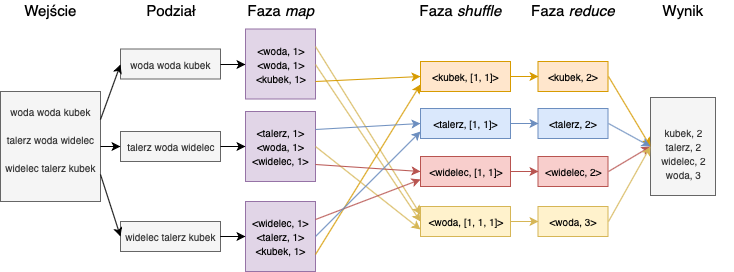
\includegraphics[width=14cm]{mapreduce_word_count.png}
\captionof{figure}{Zliczanie słów w paradygmacie MapReduce}

Dodatkowo Hadoop MapReduce zajmuje się monitorowaniem i poprawnym zarządzaniem procesami. W standardowej konfiguracji Hadoopa, Hadoop MapReduce i HDFS działają na tym samym zbiorze węzłów w klastrze. Dzięki temu możliwe jest optymalne przydzielanie procesów do danych na maszynach, co skutkuje zmniejszonym przesyłem danych oraz zwiększeniem wydajności klastra (zamiast na odwrót).

\subsection{YARN} \label{YARN}

YARN jest systemem zarządzającym zasobami oraz wykonywaniem się procesów na klastrze. Został dodany w późniejszej wersji Hadoopa (2.0), zastępując Hadoop MapReduce w kwestii zarządzania procesami i znacząco rozszerzając zakres możliwości integracji Hadoopa z~innymi modelami programistycznymi. W architekturze klastra można umieścić go pomiędzy HDFS, a serwisami odpowiedzialnymi za uruchamianie aplikacji. Zajmuje się dynamicznym przydzielaniem zasobów aplikacji, optymalizacją ich zużycia oraz uruchamianiem aplikacji.

\section{Spark}

W tym podrozdziale, opierając się na \cite{zaharia2010spark}, przedstawimy Sparka. Jest on otwartym frameworkiem pozwalającym na szybkie i efektywne przetwarzanie dużych zbiorów danych. Motywacją do stworzenia Sparka były ograniczenia stawiane przez Hadoopa w postaci intesywnego używania dysku oraz niemożliwości wykorzystania danych pośrednich na potrzeby kolejnych operacji. W Hadoopie dane można wykorzystać dopiero po ich wcześniejszym zapisaniu do HDFS. Spark natomiast umożliwia ponowne przetwarzanie cząstkowych danych bez konieczności ich zapisu, a następnie odczytu. Framework działa w oparciu o technologię \textit{in-memory}, umożliwiającą wykonywanie większości obliczeń w pamięci operacyjnej. W skład podstawowego rozwiązania Spark wchodzą:
\begin{itemize}
    \item SparkCore -- zbiór bibliotek (patrz punkt \ref{SparkCore}),
    \item Menedżer zasobów (patrz punkt \ref{Menedżer zasobów}),
    \item Rozproszony system danych (patrz punkt \ref{Rozproszony system danych}),
    \item RDD (ang. \textit{Resilient Distributed Datasets}) (patrz punkt \ref{RDD}).
\end{itemize}

Spark posiada dwa tryby przetwarzania danych: wsadowy i strumieniowy. Znajduje zastosowanie w procesach ETL, analizie danych, uczeniu maszynowym oraz algorytmach grafowych.


\subsection{SparkCore} \label{SparkCore}
SparkCore jest zbiorem bibliotek wspierającym i integrującym pozostałe moduły Sparka. Tworzy warstwę abstrakcji do zarządzania systemem. Zapewnia API wysokiego poziomu dla języków: Scala, Java, Python i R.

\subsection{Menedżer zasobów} \label{Menedżer zasobów}
Aplikacja Sparka to niezależne zbiory procesów nadzorowane i zarządzane przez obiekt \textit{SparkContext} tworzony w głównym procesie aplikacji. Na każdym węźle klastra, aplikacji zostaje przydzielony proces wykonawczy odpowiedzialny za jej uruchamianie oraz zarządzanie danymi i zasobami. Systemem zarządzającym zasobami klastra może być Spark, ale również opisany wcześniej Hadoop YARN lub podobny w działaniu Apache Mesos.

\subsection{Rozproszony system danych} \label{Rozproszony system danych}
Pomimo rozwiązania \textit{in-memory} czasem zachodzi potrzeba zapisu informacji do trwałego systemu danych. Spark wspiera szeroką gamę rozproszonych systemów przechowywania danych. Na liście znajdują się między innymi: Hadoop HDFS, Amazon S3, Cassandra czy Elasticsearch.

\subsection{Resilient Distributed Datasets} \label{RDD}
RDD to podstawowa warstwa abstrakcji danych. Jest to kolekcja obiektów, rozproszona pomiędzy węzły klastra, umożliwiająca bezpieczne i efektywne wykonywanie operacji równoległych. Główne cechy RDD to:
\begin{itemize}
    \item odporność na błędy (ang. \textit{resilient}) -- w przypadku awarii węzła klastra, Spark jest w~stanie ponownie obliczyć brakujące lub zniszczone części danych. Odtwarzanie fragmentów danych jest możliwe dzięki przechowywaniu informacji, grafu obliczeń i zależności między danymi (ang. \textit{lineage}),
    \item rozproszenie danych (ang. \textit{distributed}) -- dane kolekcji są trzymane na wielu węzłach klastra jednocześnie,
    \item kolekcjonowanie danych (ang. \textit{dataset}) -- RDD przechowuje obiekty wszelkiego rodzaju, począwszy od typów podstawowych, aż do złożonych rekordów danych,
    \item zrównoleglenie -- obliczenia i przekształcenia wykonywane są w sposób równoległy,
    \item \textit{in-memory} i utrwalanie danych -- RDD jest traktowane jak regularny obiekt, zatem jest przechowywane w pamięci operacyjnej tak długo jak to potrzebne. Istnieje możliwość trwałego zapisu RDD do pamięci podręcznej lub zintegrowanego systemu przechowywania danych, zapewniając tym samym szybszy dostęp do danych pomiędzy procesami,
    \item leniwa ewaluacja -- dane zawarte w RDD nie są dostępne i przetwarzane do momentu wywołania akcji,
    \item stałość -- raz stworzone RDD nie może być zmienione, może być jedynie przekształcone w nowe RDD.
    
\end{itemize}

RDD wspierają dwa typy operacji:
\begin{itemize}
    \item \textit{przekształcenia / transformacje} -- leniwie wykonywane obliczenia i operacje zwracające nowe RDD np: \textit{map}, \textit{filter}, \textit{join},
    \item \textit{akcje} -- obliczenia wykonywane na RDD i zwracające wynik np: \textit{reduce}, \textit{count}.
\end{itemize}

Podstawową jednostką RDD jest partycja, która jest logiczną częścią rozproszonego zbioru danych. Liczbę partycji można kontrolować. Spark optymalizuje przesył danych przez sieć, przez co stara się odtworzyć logiczny podział danych na ich fizyczne odpowiedniki.

Stworzenie RDD umożliwiło efektywne implementowanie:
\begin{itemize}
    \item interaktywnych narzędzi do analizy danych i wykonywania zapytań,
    \item iteracyjnych algorytmów używanych w uczeniu maszynowym czy analizie grafów.
\end{itemize}

\section{Hadoop vs Spark}

Hadoop powstał na trzy lata przed Sparkiem i przez ten czas bardzo dobrze spisywał się jako framework do przetwarzania dużych danych. MapReduce spełniał swoją funkcję jako paradygmat liniowego przetwarzania danych. Jednak z upływem czasu pojawiły się nowe potrzeby, dla których Hadoop nie był dopasowany. Napisanie skomplikowanego algorytmu przy użyciu MapReduce jest czasochłonne. Dodatkowo zaimplementowane rozwiązanie jest zazwyczaj wolne z powodu wielu kroków pośrednich, z których każdy zostaje zapisany do HDFS. W celu usprawnienia powyższych aspektów został stworzony Spark. Umożliwia on pisanie efektywnych i skomplikowanych algorytmów rozproszonych. Używanie grafów wykonań oraz technologii \textit{in-memory} znacząco zredukowało czas wykonania programów. Na \mbox{Rysunku 2.2} przedstawiono wykres porównujący rezultaty sortowania danych przy użyciu Hadoop MapReduce i Sparka. Program napisany w Sparku posortował dane 3 razy szybciej, używając 10 razy mniej maszyn.


\begin{figure}[H]
    \caption{Porównanie rekordów Hadoopa (2013) i Sparka (2014) w sortowaniu 100 TB danych używając testu wydajności \textit{Daytona Gray} \cite{Armbrust:2015:SSR:2824032.2824080}.}
    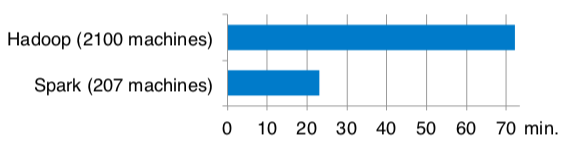
\includegraphics[width=15cm]{hadoop_vs_spark.png}
\end{figure}

Dodatkowo Spark udostępnia bardzo rozbudowane API do języków Scala, Java, Python i R. W przeciwieństwie do Hadoopa, tworzenie nowych algorytmów jest intuicyjne, łatwe i szybkie. Oba frameworki posiadają cały szereg zintegrowanych systemów ułatwiających przetwarzanie dużych danych, jednak to Spark jest obecnie bardziej rozwijanym projektem.

\chapter{Algorytmy minimalne}\label{algorytmy_minimalne}
\section{Definicja}

Oznaczmy \textit{S} jako zbiór obiektów w rozpatrywanym problemie. Niech \textit{n} będzie liczbą obiektów wchodzących w skład \textit{S}, a \textit{t} liczbą maszyn w systemie. Zdefiniujmy \textit{m = n/t}, czyli liczbę obiektów na każdej z maszyn w przypadku równomiernego rozproszenia \textit{S}. Rozważmy algorytm rozwiązujący pewien problem na zbiorze \textit{S}. Mówimy, że algorytm jest \textit{minimalny} jeżeli posiada wszystkie z następujących własności \cite{tao2013minimal}:
\begin{itemize}
    \item \textit{ograniczona pamięć} -- każda z maszyn zużywa \textit{O(m)} pamięci,
    \item \textit{ograniczony przesył danych} -- w każdej rundzie MapReduce / transformacji RDD, każda z maszyn wysyła i odbiera przez sieć co najwyżej \textit{O(m)} informacji,
    \item \textit{stała liczba rund} -- algorytm musi zakończyć się po stałej liczbie rund / transformacji RDD,
    \item \textit{optymalność obliczeń} -- każda maszyna wykonuje \(O(T_{seq} / t\)) obliczeń, gdzie \(T_{seq}\) jest czasem potrzebnym na rozwiązanie problemu na pojedynczej maszynie sekwencyjnej. Mianowicie algorytm powinien otrzymać przyspieszenie rzędu \(t\), używając równolegle \(t\)~maszyn.
\end{itemize}

Fazy i rundy MapReduce oraz transformacje RDD są w stanie wyrazić dowolne obliczenia rozproszone \cite{zaharia2016apache}. Oznacza to również, że obliczenia wykonywane w paradygmacie MapReduce można wyrazić przekształceniami RDD i odwrotnie. Z tego powodu opisy przedstawionych algorytmów minimalnych zostały zapisane tylko w paradygmacie MapReduce.
\section{TeraSort} \label{tera_sort}

TeraSort jest rozproszonym algorytmem sortującym. Na wejściu mamy dany zbiór \(S\) składający się z \(n\) porównywalnych obiektów. Do dyspozycji mamy \(t\) maszyn \(M_1, ..., M_t\). Początkowo zbiór \(S\) jest równomiernie rozproszony na maszynach. Rezultatem algorytmu jest stan, w którym obiekty na maszynie \(M_i\) są posortowane oraz poprzedzają obiekty na maszynach \(M_j\) dla każdego \(1 \leq i < j \leq t\). Parametryzowany zmienną \(\rho \in (0, 1]\) algorytm TeraSort składa się z następujących faz MapReduce \cite{tao2013minimal}:\\

\enlargethispage{-\baselineskip}
\enlargethispage{-\baselineskip}
\enlargethispage{-\baselineskip}
\textbf{Runda 1}
\begin{itemize}
    \item \textit{Map-shuffle} \\
    Na każdej z maszyn \(M_i\) (\(1 \leq i \leq t)\), odczytujemy z pamięci lokalnej obiekty wejściowe algorytmu i każdy z nich wybieramy z prawdopodobieństwem \(\rho = \frac{1}{m}\ln(nt)\) \cite{tao2013minimal}. Na koniec wysyłamy wybrane elementy na wszystkie maszyny \(M_1, ..., M_t\).
    \item \textit{Reduce} \\
    Niech \(S^{\prime}\) oznacza zbiór elementów otrzymanych z fazy \(map\), a \(s^{\prime} = |S^{\prime}|\). Początkowo sortujemy \(S^{\prime}\), a następnie wybieramy obiekty graniczne \(b_1, ..., b_{t-1}\), gdzie \(b_i\) jest obiektem o indeksie \(i*\lceil{s^{\prime} / t}\rceil\) dla \(1 \leq i \leq t-1\).
\end{itemize}

\textbf{Runda 2}
\begin{itemize}
    \item \textit{Map-shuffle} \\
    Każda maszyna \(M_i\) odczytuje z pamięci lokalnej początkowe obiekty i wysyła elementy należące do przedziału \((b_{j-1}, b_j]\) na maszynę \(M_j\), dla każdego \(1 \leq j \leq t\), gdzie \(b_0 = -\infty\) oraz \(b_t = \infty\).
    \item \textit{Reduce} \\
    Każda maszyna \(M_i\) sortuje obiekty otrzymane z fazy \(map\).
\end{itemize}


\section{Lista rankingowa} \label{list_rankingowa}

Niech \(S\) oznacza zbiór \(n\) porównywalnych obiektów wejściowych. Rezultatem algorytmu jest zwrócenie pozycji rankingowej \(rank(o) = |\{o^\prime \in S : \ o^\prime \leq o\}|\), dla każdego \(o \in S\). Problem można rozwiązać w czasie \textit{O(n log n)} na pojedynczej maszynie. Przykładowo dla \(S = \{4, 8, 1, 7, 10\}\) lista rankingowa prezentuje się następująco:
\begin{flalign*}
rank(1) &= 1\\
rank(4) &= 2\\
rank(7) &= 3\\
rank(8) &= 4\\
rank(10) &= 5\\
\end{flalign*}
Poniżej została przedstawiona rozproszona wersja algorytmu w oparciu o paradygmat MapReduce \cite{tao2013minimal}. \\

\textbf{Rundy 1 -- 2} \\
Sortujemy \(S\) przy użyciu algorytmu \(TeraSort\). \\

\textbf{Runda 3} \\
Niech \(Sorted_i\) oznacza posortowany zbiór obiektów na maszynie \(M_i\), dla \(1 \leq i \leq t\).
\begin{itemize}
    \item \textit{Map-shuffle} \\
    Każda maszyna \(M_i\) wysyła \(|Sorted_i|\) na maszyny \(M_{i+1}, ..., M_t\).
    \newpage
    \item \textit{Reduce} \\
    Niech:
    \begin{itemize}
        \item $R_i = \sum_{j \leq i-1} \ |Sorted_j|$
        \item \(localRank(o) = |\{o^\prime \in Sorted_i : \ o^\prime \leq o\}|\) dla każdego \(o \in Sorted_i\)
    \end{itemize}
    Numer rankingowy wynosi: \\
    $$rank(o) = R_i + localRank(o)$$
    
\end{itemize}

\section{Statystyki prefiksowe} \label{statystyki_prefiksowe}
Niech \(S\) oznacza zbiór \(n\) porównywalnych obiektów wejściowych, a \(stat\) będzie funkcją statystyk łączną na zbiorze \(S\). Z łączności wynika zatem, że \(stat(S)\) może zostać obliczone w~czasie stałym ze \(stat(S_1)\) i \(stat(S_2)\), gdzie \(S_1\) i \(S_2\) tworzą podział \(S\), czyli \(S_1 \cup S_2 = S\) oraz \(S_1 \cap S_2 = \emptyset\). Rezultat algorytmu definiujemy następująco \cite{tao2013minimal}:
\begin{center}
\(prefixStat(o, stat) = stat(\{o^\prime \in S: \ o^\prime < o\})\) dla każdego \(o \in S\) \\
\end{center}

Przykładową funkcją \(stat\) jest \(suma\). Niech \(S = \{1, 2, 3, 4\}\), wtedy
\begin{flalign*}
prefixStat(1, suma) &= suma(\emptyset) = 0\\
prefixStat(2, suma) &= suma(\{1\}) = 1\\
prefixStat(3, suma) &= suma(\{1, 2\}) = 1 + 2 = 3\\
prefixStat(4, suma) &= suma(\{1, 2, 3\}) = 1 + 2 + 3 = 6
\end{flalign*}

\textbf{Rundy 1 -- 2} \\
Sortujemy \(S\) przy użyciu algorytmu \(TeraSort\). \\

\textbf{Runda 3} \\
Niech \(Sorted_i\) oznacza posortowany zbiór obiektów na maszynie \(M_i\), dla \(1 \leq i \leq t\).
\begin{itemize}
    \item \textit{Map-shuffle} \\
    Każda maszyna \(M_i\) wysyła \(stat(Sorted_i)\) na maszyny \(M_{i+1}, ..., M_t\).
    \item \textit{Reduce} \\
    Niech
    \begin{itemize}
        \item \(V_i = stat(\{stat(Sorted_1), stat(Sorted_2),..., stat(Sorted_{i-1})\})\)
        \item \(prefixLocal(o, stat) = stat(\{o^\prime \in Sorted_i: \ o^\prime < o \})\) dla każdego \(o \in Sorted_i\)
    \end{itemize}
    Statystyki prefiksowe wynoszą: \\
    
    \centering
    \(prefixStat(o, stat) = V_i + prefixLocal(o, stat)\) dla każdego \(o \in Sorted_i\)
\end{itemize}

\section{Grupowanie}
Niech \(S\) oznacza zbiór \(n\) porównywalnych obiektów wejściowych, a \(stat\) będzie funkcją statystyk łączną na zbiorze \(S\). Dodatkowo dla każdego \(o \in S\) istnieje funkcja \(key(o)\) zwracająca obiekt będący porównywalnym kluczem danego elementu \(o\). Grupą \(G\) nazwiemy maksymalny zbiór obiektów, dla których funkcja \(key\) zwraca tą samą wartość.
\newpage
Rezultat algorytmu \textit{grupowania} definiujemy następująco \cite{tao2013minimal}:
\begin{center}
\(groupBy(G, stat) = stat(G)\) dla każdej grupy \(G\) na zbiorze \(S\) \\
\end{center}

Przykładowo niech funkcją \(stat\) będzie \(suma\), \(S = \{1, 2, 3, 4, 5\}\) oraz
\begin{flalign*}
key(1) &= 42\\
key(2) &= 42\\
key(3) &= 35\\
key(4) &= 35\\
key(5) &= 42
\end{flalign*}

Następnie wyznaczamy grupy:
\begin{flalign*}
G_{42} &= \{1, 2, 5\}\\
G_{35} &= \{3, 4\}
\end{flalign*}

Końcowy wynik algorytmu wynosi:
\begin{flalign*}
groupBy(G_{42}, suma) &= suma(\{1, 2, 5\}) = 8\\
groupBy(G_{35}, suma) &= suma(\{3, 4\}) = 7
\end{flalign*}

\textbf{Rundy 1 -- 2} \\
Sortujemy \(S\) przy użyciu algorytmu \(TeraSort\). \\

\textbf{Runda 3} \\
Niech \(Sorted_i\) oznacza posortowany zbiór obiektów na maszynie \(M_i\), dla \(1 \leq i \leq t\).

\begin{itemize}
    \item \textit{Map-shuffle} \\
    Niech:
    \begin{itemize}
        \item \(k_{min}(i) = min(\{key(o) : \ o \in Sorted_i \})\)
        \item \(k_{max}(i) = max(\{key(o) : \ o \in Sorted_i \})\)
    \end{itemize}
    
    Jeżeli dla danego klucza \(k\), grupa \(G_{k}\) znajduje się całkowicie na \mbox{maszynie \(M_i\)}, to \(groupBy(G_{k}, stat)\) obliczamy lokalnie na  \(M_i\), a następnie przesyłamy parę \((k, groupBy(G_{k}, stat))\) na maszynę \(M_i\). Takie grupy są tworzone przez obiekty \mbox{\(o \in Sorted_i\)}, takie że \(k_{min}(i) < key(o) < k_{max}(i)\). Wynika z tego, że każda maszyna \(M_i\) ma co najwyżej dwie grupy, które nie mogą zostać obliczone lokalnie:
    \begin{center}
    \(G_{min}(i) = \{o : \ o \in Sorted_i \wedge key(o) = k_{min}(i)\}\) \\
    \(G_{max}(i) = \{o : \ o \in Sorted_i \wedge key(o) = k_{max}(i)\}\) \\
    \end{center}
    
    Stąd wiadomo, że takich grup na wszystkich maszynach jest maksymalnie \(2t\). Aby obliczyć wynik dla grup niemieszczących się na pojedynczej maszynie, najpierw obliczamy \(stat(G_{min}(i))\) oraz \(stat(G_{max}(i))\) lokalnie na \(M_i\). Następnie wybieramy pojedynczą maszynę, np. \(M_1\), na której zgrupujemy lokalne wyniki. W ostatnim kroku wysyłamy parę \((k_{min}(i), stat(G_{min}(i)))\) na wybraną maszynę \(M_1\) oraz jeżeli \(k_{min}(i) \neq k_{max}(i)\), to wysyłamy również parę \((k_{max}(i), stat(G_{max}(i)))\) na maszynę \(M_1\). Widzimy, że policzenie statystyk na takich grupach wymaga przesłania dwóch lub czterech wartości na pojedynczą maszynę, na której zostanie obliczony końcowy wynik.

    \item \textit{Reduce} \\
    Na maszynach \(M_2, ..., M_t\) mamy już gotowe wyniki grupowania. Natomiast na wybranej maszynie \(M_1\) niech \((k_1, w_1), ..., (k_x, w_x)\) oznaczają pary otrzymane z fazy \(map\), gdzie \(x \in [t, 2t]\). Dla każdej grupy, której klucz \(k\) jest wśród otrzymanych par, wynikiem algorytmu jest:\\
            $$G_k = stat(\{w_j: \ k = k_j\})$$
\end{itemize}
\section{Pół-złączenia}
Niech \(R\) i \(T\) będą dwoma zbiorami z tej samej dziedziny. Dla każdego obiektu \(o \in R \ \cup \  T\) istnieje funkcja \(key(o)\) zwracająca klucz obiektu \(o\). Problem \textit{pół-złączeń} polega na znalezieniu wszystkich obiektów \(o \in R\), takich że istnieje obiekt \(o^\prime \in T\), dla którego \(key(o) = key(o^\prime)\). Zakładamy również, że elementy zbiorów są zdefiniowane w sposób pozwalający na rozróżnienie, z którego zbioru pochodzą. Problem pół-złączeń posiada rozwiązanie o złożoności czasowej \(O(n \ log \  n)\) na pojedynczej maszynie sekwencyjnej, gdzie \(n = |R \cup T|\) \cite{tao2013minimal}.\\

Przykładowo niech \(R = \{1, 2, 5\}\), \(T = \{7, 8, 9\}\) oraz
\begin{flalign*}
key(1) &= 20 \ \ \ \ \ key(7) = 21\\
key(2) &= 21 \ \ \ \ \ key(8) = 23\\
key(5) &= 22 \ \ \ \ \ key(9 )= 20\\
\end{flalign*}
Wynikiem algorytmu jest zbiór \(\{1, 2\}\), ponieważ \(key(1) = key(9)\) oraz \(key(2) = key(7)\). \\

\textbf{Rundy 1 -- 2} \\
Sortujemy \(R \cup T\) przy użyciu algorytmu \(TeraSort\). \\

\textbf{Runda 3} \\
Zdefiniujmy \(R_i\) oraz \(T_i\) jako zbiory obiektów znajdujących się na maszynie \(M_i\) i początkowo należących odpowiednio do zbiorów \(R\), \(T\).

\enlargethispage{-\baselineskip}
\enlargethispage{-\baselineskip}
\enlargethispage{-\baselineskip}

\begin{itemize}
    \item \textit{Map-shuffle} \\
    Na każdej maszynie \(M_i\), dla \(1 \leq i \leq t\), wysyłamy do wszystkich maszyn następujące dwie wartości:
        \begin{itemize}
            \item \(min(\{key(o): o \in T_i\})\),
            \item \(max(\{key(o): o \in T_i\})\).
        \end{itemize}
    \item \textit{Reduce} \\
    Niech \(T_{border}\) będzie zbiorem kluczy otrzymanych z fazy \(map\). Na każdej z maszyn \(M_i\), dla \(1 \leq i \leq t\), zwracamy obiekt \(o \in R_i\) jako część rezultatu, gdy
            $$key(o) \in T_i \cup T_{border}$$

\end{itemize}

\section{Sortowanie z perfekcyjnym zrównoważeniem} \label{perfect_sort}

Niech \(S\) będzie zbiorem składającym się z \(n\) porównywalnych obiektów, a \(m = \lceil n / t \rceil\). Aby otrzymać rezultat algorytmu, należy przegrupować elementy, tak aby każda z maszyn \(M_1, ..., M_{t-1}\) zawierała dokładnie \(m\) obiektów, a maszyna \(M_t\) zawierała pozostałe. Dodatkowo obiekty na maszynie \(M_i\), dla \(1 \leq i \leq t\), są posortowane oraz poprzedzają obiekty na maszynach \(M_j\) dla \(1 \leq i < j \leq t\).\\

\textbf{Rundy 1 -- 3} \\
Na zbiorze \(S\) wykonujemy algorytm \textit{listy rankingowej}. Niech \(rank(o)\) dla \(o \in S\) oznacza pozycję rankingową obiektu \(o\). \\

\textbf{Runda 4} \\
Wykonujemy tylko fazę \textit{map-shuffle}, w której dla każdego obiektu \(o\) na maszynie \(M_i\), dla \(1 \leq i \leq t\), wysyłamy go na maszynę \(M_j\), gdzie \(j = \lceil rank(o) / m \rceil\).

\section{Statystyka okienkowa}
Niech:
\begin{itemize}
    \item \(S\) -- zbiór \(n\) porównywalnych obiektów,
    \item \(l\) -- wielkość okna statystyk, \(l \leq n\),
    \item \(stat\) -- funkcja statystyk łączna na zbiorze \(S\).
\end{itemize}

Dla każdego \(o \in S\) zdefiniujmy \(window(o)\) jako zbiór \(l\) największych obiektów nie przekraczających \(o\). Statystyka okienkowa obiektu \(o\) wynosi:
$$winStat(o) = stat(window(o))$$

Rezultatem algorytmu \textit{statystyki okienkowej} \cite{tao2013minimal} jest zwrócenie wartości \(winStat(o)\) dla każdego obiektu \(o \in S\). \\

Przykładowo dla \(S = \{1, 2, 3, 4, 5\}\), \(l = 3\) oraz \(stat = suma\) wynikiem algorytmu jest:
\begin{flalign*}
winStat(1) &= suma(\{1\}) = 1 \\
winStat(2) &= suma(\{1, 2\}) = 3 \\
winStat(3) &= suma(\{1, 2, 3\}) = 6 \\
winStat(4) &= suma(\{2, 3, 4\}) = 9 \\
winStat(5) &= suma(\{3, 4, 5\}) = 12 \\
\end{flalign*}

\textbf{Rundy 1 -- 4} \\
Wykonujemy algorytm \textit{sortowania z perfekcyjnym zrównoważeniem}. W dalszej części algorytmu \(m = \lceil n / t \rceil\). \\
\newpage
\textbf{Runda 5} \\
Niech \(S_i\) oznacza zbiór elementów na maszynie \(M_i\), dla \(1 \leq i \leq t\).

\begin{itemize}
    \item \textit{Map-shuffle} \\
     Do wszystkich maszyn wysyłamy \(W_i = stat(S_i)\). Następnie, zgodnie z lematem \(2\) z~\mbox{pracy \cite{tao2013minimal}}, każdy obiekt \(o \in S_i\) musi zostać wysłany na maksymalnie dwie dodatkowe maszyny. Zatem przesyłamy wszystkie obiekty zbioru \(S_i\) na maszynę \(M_{i+1}\), jeżeli \(l \leq m\), a w przeciwnym przypadku na maszyny o indeksach \(i + \lfloor (l - 1) / m \rfloor\) oraz \(i+1+\lfloor (l-1)/m \rfloor \).
    
    \item \textit{Reduce} \\
    Dla każdego \(o \in S_i\) obliczamy:
    \begin{itemize}
        \item \(\alpha = \lceil (rank(o) - l + 1) / m \rceil\),
        \item \(w_1 = stat(\{o^\prime : o^\prime \in S_\alpha \wedge o^\prime \in window(o)\})\). Jeżeli \(\alpha < i \), to takie obiekty \(o^\prime\) zostały przysłane na maszynę \(M_i\) w fazie \textit{map-shuffle} rundy 5,
        \item $w_2 = \sum_{j=\alpha+1}^{i-1} W_j$,
        \item jeżeli \(\alpha = i\), to \(w_3 = 0\), wpp \(w_3 = stat(\{o^\prime : o^\prime \in S_i \wedge o^\prime \in window(o)\})\).
    \end{itemize}
    
    $$winStat(o) = stat(\{w_1, w_2, w_3\})$$
\end{itemize}

 Na Rysunku 3.1 przedstawiono przykład działania rundy 5 dla maszyny \(i = 5\). Niech \(o_{r}\) oznacza obiekt \(o \in S\) z pozycją rankingową równą \(r\) oraz \(l = 35, m = 10\).

\begin{figure}[H]
    \caption{Rozesłanie obiektów podczas rundy 5 algorytmu agregacji okienkowej}
    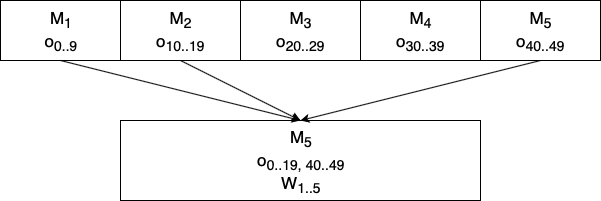
\includegraphics[width=15cm]{sliding_agg.png}
\end{figure}

Wartość agregacji okienkowej dla \(o_{42}\) obliczamy następująco:
\begin{flalign*}
\alpha &= 1\\
w_1 &= stat(\{o_8, o_9\})\\
w_2 &= stat(\{W_2, W_3, W_4\})\\
w_3 &= stat(\{o_{40}, o_{41}, o_{42}\})\\
winStat(o_{42}) &= stat(\{w_1, w_2, w_3\}
\end{flalign*}

\chapter{Biblioteka do tworzenia algorytmów minimalnych}
\setlength{\parindent}{6.5ex}
Z rozdziału \ref{algorytmy_minimalne} wynika jak dużo wspólnych obliczeń i funkcjonalności posiadają poszczególne algorytmy minimalne. Należą do nich między innymi sortowanie obiektów, liczenie łącznych statystyk na zbiorach, wysyłanie obiektów na wybrane maszyny oraz równolegle przesyłanie wielu typów obiektów. W poniższym rozdziale przedstawię implementację mojej biblioteki, napotkane problemy i ich rozwiązania. Podrozdziały Hadoop \ref{hadoop} oraz Spark \ref{spark} przedstawiają kolejno:
\begin{enumerate}
    \item Implementację algorytmu minimalnego bez użycia biblioteki,
    \item Implementację algorytmu minimalnego z użyciem biblioteki,
    \item Opis implementacji biblioteki.
\end{enumerate}

\section{Wstęp}
\textit{MinimalAlgFactory} jest klasą udostępniającą zaimplementowane algorytmy minimalne. Została napisana w języku Java 8. Jej zadaniem jest połączenie implementacji algorytmów minimalnych na platformy Hadoop i Spark. Dzięki takiemu rozwiązaniu użytkownik może raz napisany algorytm uruchamiać na jednym z frameworków bez konieczności dostosowywania. W skład klasy wchodzą algorytmy:
\begin{itemize}
    \item \textit{TeraSort} -- sortowanie,
    \item \textit{Rank} -- lista rankingowa,
    \item \textit{PerfectSort} -- sortowanie z perfekcyjnym równoważeniem,
    \item \textit{Prefix} -- statystyki prefiksowe,
    \item \textit{SemiJoin} -- pół-złączenia,
    \item \textit{GroupBy} -- grupowanie,
    \item \textit{SlidingAggregation} -- statystyka okienkowa.
\end{itemize}

\section{Hadoop} \label{hadoop}

\subsection{Implementacja algorytmu bez użycia biblioteki} \label{hbub}

Listingi \ref{list_four_ints} -- \ref{list_prefix} przedstawiają implementację algorytmu statystyk prefiksowych przy użyciu podstawowej wersji Hadoopa 2.8. Funkcją statystyk jest suma. Na Listingu \ref{list_four_ints} ukazano klasę obiektów wejściowych. W plikach z danymi każda linia składa się z czterech liczb całkowitych oddzielonych spacją i reprezentuje pojedynczy obiekt klasy \(FourInts\). W liniach 22 -- 24 została zaimplementowana funkcja obliczającą wartość obiektu, która będzie wykorzystywana w liczeniu sum prefiksowych. Natomiast linie 35 -- 42 przedstawiają komparator użyty do porównywania obiektów \(FourInts\).

\begin{lstlisting}[language=SmallJava,firstnumber=1,label=list_four_ints,caption=Klasa danych wejściowych do algorytmu statystyk prefiksowych]
public class FourInts {
  public static final String DELIMITER = " ";
  private int first;
  private int second;
  private int third;
  private int fourth;
  private String encodedValues;

  public FourInts(String encodedValues) {
    this.encodedValues = encodedValues;
    String[] values = encodedValues.split(DELIMITER);
    this.first = Integer.parseInt(values[0]);
    this.second = Integer.parseInt(values[1]);
    this.third = Integer.parseInt(values[2]);
    this.fourth = Integer.parseInt(values[3]);
  }

  public FourInts(Text encodedValues) {
    this(encodedValues.toString());
  }

  public long getValue() {
    return this.second + this.third + this.fourth;
  }

  @Override
  public String toString() {
    return this.encodedValues;
  }

  public Text toText() {
    return new Text(this.toString());
  }

  public static class FourIntsComparator implements Comparator<FourInts> {
    @Override
    public int compare(FourInts o1, FourInts o2) {
      return o1.first > o2.first ? 1 : (o1.first < o2.first ? -1 : 0);
    }
  }

  public static Comparator<FourInts> cmp = new FourIntsComparator();
}
\end{lstlisting}

\newpage 
Klasa \(MultipleFourInts\) z Listingu \ref{list_multi_four_ints} przedstawia prosty serializator kolekcji obiektów \(FourInts\). Zostanie wykorzystana przy implementacji rund algorytmu \mbox{na Listingach \ref{list_sampling} -- \ref{list_prefix}}.

\begin{lstlisting}[language=SmallJava,firstnumber=1,label=list_multi_four_ints,caption=Kolekcja obiektów FourInts]
public class MultipleFourInts {
  public static final String DELIMITER = "#";
  private List<FourInts> fourIntsSeq;

  public MultipleFourInts(Text encodedValues){
    this(encodedValues.toString());
  }

  public MultipleFourInts(String encodedValues) {
    this.fourIntsSeq = new ArrayList<>();
    for (String value : encodedValues.split(DELIMITER)) {
      this.fourIntsSeq.add(new FourInts(value));
    }
  }

  public MultipleFourInts(List<FourInts> fourIntsSeq) {
    this.fourIntsSeq = fourIntsSeq;
  }

  public List<FourInts> getValues() {
    return this.fourIntsSeq;
  }

  @Override
  public String toString() {
    List<String> result = new ArrayList();
    for (FourInts fourInts : this.fourIntsSeq) {
      result.add(fourInts.toString());
    }
    return String.join(DELIMITER, result);
  }

  public Text toText() {
    return new Text(this.toString());
  }
}
\end{lstlisting}

\newpage
Listing \ref{list_index_stats} przedstawia klasę, w której trzymane są statystyki dla całych maszyn. Atrybut \(key\) oznacza numer maszyny, z której pochodzą statystyki, a atrybut \(statistics\) oznacza wartość sumy obiektów na danej maszynie. W liniach 21 -- 33 zdefiniowano komparator, umożliwiający posortowanie statystyk względem numerów maszyn.

\begin{lstlisting}[language=SmallJava,firstnumber=1,label=list_index_stats,caption=Klasa indeksowanych statystyk]
public class IndexedStatistics {
  public static final String DELIMITER = "%";
  public int key;
  public long statistics;
  public String encodedValue;

  public IndexedStatistics(String key, long statistics) {
    this.encodedValue = key + DELIMITER + Long.toString(statistics);
  }

  public IndexedStatistics(Text encodedValue) {
    String[] tokens = encodedValue.toString().split(DELIMITER);
    this.key = Integer.parseInt(tokens[0]);
    this.statistics = Long.parseLong(tokens[1]);
  }

  public Text toText() {
    return new Text(this.encodedValue);
  }

  public static class IndexedStatisticsComparator
        implements Comparator<IndexedStatistics> {
    @Override
    public int compare(IndexedStatistics o1, IndexedStatistics o2) {
      return o1.key > o2.key ?
        1 : (o1.key < o2.key ?
          -1 : (o1.statistics > o2.statistics ?
            1 : o1.statistics < o2.statistics ? -1 : 0));
    }
  }

  public static Comparator<IndexedStatistics> cmp =
    new IndexedStatisticsComparator();
}
\end{lstlisting}

\newpage
Na Listingu \ref{list_run_prefix_app} widzimy klasę uruchamiającą algorytm. W liniach 17 -- 24 przygotowujemy konfigurację programu, dostępną przez cały czas wykonania programu, w każdej fazie \(map\) i \(reduce\). Jest to standardowy sposób udostępniania niewielkich wartości wszystkim maszynom. Następnie w liniach 27 -- 31 uruchamiamy kolejne rundy algorytmu. Widzimy, że danymi wejściowymi do kolejnych rund są wyniki poprzednich.

\begin{lstlisting}[language=SmallJava,firstnumber=1,label=list_run_prefix_app,caption=Uruchamianie algorytmu]
public class PrefixApp extends Configured implements Tool {
  private int computeRatioRandom(int itemsNo, int partitionsNo) {
    int itemsPerPartition = 1 + itemsNo / partitionsNo;
    double rho = 1. / itemsPerPartition *
      Math.log(((double) itemsNo) * partitionsNo);
    return (int) (1 / rho);
  }

  public int run(String[] args) throws Exception {
    if (args.length != 6) {
      System.err.println("Usage: PrefixApp" +
        "<home_dir> <input_path> <output_path>" +
        "<items_no> <partitions_no> <reduce_tasks_no>");
      return -1;
    }

    Configuration conf = getConf();
    int itemsNo = Integer.parseInt(args[3]);
    int partitionsNo = Integer.parseInt(args[4]);
    int reducersNo = Integer.parseInt(args[5]);
    
    conf.setInt(Utils.RATIO_KEY, computeRatioRandom(itemsNo, partitionsNo));
    conf.setInt(Utils.SPLIT_POINTS_KEY, partitionsNo);
    conf.setInt(Utils.REDUCERS_NO_KEY, reducersNo);
    
    Path input = new Path(args[1]);
    Sampling.run(input, new Path("samp"), conf);
    Sorting.run(input, new Path(args[0] + "/samp"), new Path("sort"), conf);
    PartStats.run(new Path(args[0] + "/sort"), new Path("part_stats"), conf);
    return Prefix.run(new Path(args[0] + "/sort"),
        new Path(args[0] + "/part_stats"), new Path("prefix"), conf);
  }

  public static void main(String[] args) throws Exception {
    int res = ToolRunner.run(new Configuration(), new PrefixApp(), args);
    System.exit(res);
  }
}
\end{lstlisting}

\newpage
Przed wykonaniem faz \(map\) i \(reduce\) Hadoop MapReduce umożliwia zapisanie danych w postaci tekstowej do lokalnego systemu plików każdego \(DataNode\) -- funkcja \(addCacheFile\). Klasa \(Utils\) z Listingu \ref{list_utils} udostępnia pomocniczą metodę odczytywania obiektów z tak zapisanych plików. Pozwala to na szybki dostęp do niedużych obiektów niezbędnych na każdej maszynie.

\begin{lstlisting}[language=SmallJava,firstnumber=1,label=list_utils,caption=Metody pomocniczne]
public class Utils {
  public static final String RATIO_KEY = "ratio";
  public static final String SPLIT_POINTS_KEY = "splitPoints";
  public static final String REDUCERS_NO_KEY = "reducersNo";

  public static ArrayList<String> readFromCache(Path filePath) {
    ArrayList<String> words = new ArrayList<>();
    try {
      BufferedReader bufferedReader = new BufferedReader(
        new FileReader(filePath.toString()));
      String word = null;
      while((word = bufferedReader.readLine()) != null) {
        words.add(word);
      }
    } catch(IOException ex) {
      System.err.println(ex.getMessage());
    }
    return words;
  }
}
\end{lstlisting}

Na Listingu \ref{list_sampling} przedstawiono pierwszą rundę algorytmu \(TeraSort\). W linii 10 odczytujemy z konfiguracji, uzupełnionej przy uruchomieniu programu, wartość prawdopodobieństwa \(\rho\) zdefiniowanego w podrozdziale \ref{tera_sort}. Następnie w liniach 16 -- 18 wybieramy obiekty wejściowe z prawdopodobieństwem \(\rho\) i wysyłamy na jedną z maszyn. Warto zauważyć, że w~celu wysłania wszystkich wybranych obiektów na jedną maszynę używamy klucza o wartości NULL.

W fazie \(reduce\) odbieramy wybrane obiekty i parsujemy do typu \(FourInts\). Następnie sortujemy i wyznaczamy miejsca podziałów. Warto zauważyć, że w linii 53 ustawiamy ilość reducerów na 1, dzięki czemu wszystkie miejsca podziałow znajdą się w jednym pliku.

\begin{lstlisting}[language=SmallJava,firstnumber=1,label=list_sampling,caption=Faza próbkowania danych]
public class Sampling {
  public static class SamplerMapper extends
        Mapper<LongWritable, Text, NullWritable, Text> {
    private final Random random = new Random();
    private int ratioForRandom;

    @Override
    public void setup(Context ctx) throws IOException, InterruptedException {
      super.setup(ctx);
      ratioForRandom = ctx.getConfiguration().getInt(Utils.RATIO_KEY, -1);
    }

    @Override
    public void map(LongWritable key, Text value, Context context) throws
        IOException, InterruptedException {
      if (random.nextInt(ratioForRandom) == 0) {
        context.write(NullWritable.get(), value);
      }
    }
  }

  public static class ComputeBoundsForSortingReducer extends
        Reducer<NullWritable, Text, Text, NullWritable> {
    private int noOfSplitPoints;

    @Override
    public void setup(Context ctx) throws IOException, InterruptedException {
      super.setup(ctx);
      Configuration conf = ctx.getConfiguration();
      noOfSplitPoints = conf.getInt(Utils.SPLIT_POINTS_KEY, 0) - 1;
    }

    @Override
    protected void reduce(NullWritable key, Iterable<Text> values,
        Context context) throws IOException, InterruptedException {
      ArrayList<FourInts> result = new ArrayList<>();
      for (Text value : values) {
        result.add(new FourInts(value));
      }

      java.util.Collections.sort(result, FourInts.cmp);
      int step = result.size() / (noOfSplitPoints+1);
      for (int i = 1; i <= noOfSplitPoints; i++) {
        context.write(result.get(i * step).toText(), NullWritable.get());
      }
    }
  }

  public static int run(Path input, Path output, Configuration conf) throws
        IOException, InterruptedException, ClassNotFoundException {
    Job job = Job.getInstance(conf, "JOB: Phase sampling");
    job.setJarByClass(Sampling.class);
    job.setNumReduceTasks(1);

    FileInputFormat.setInputPaths(job, input);
    FileOutputFormat.setOutputPath(job, output);

    job.setMapperClass(SamplerMapper.class);
    job.setReducerClass(ComputeBoundsForSortingReducer.class);

    job.setMapOutputKeyClass(NullWritable.class);
    job.setMapOutputValueClass(Text.class);
    job.setOutputKeyClass(Text.class);
    job.setOutputValueClass(NullWritable.class);

    return job.waitForCompletion(true) ? 0 : 1;
  }
}
\end{lstlisting}

\newpage
Listing \ref{list_sorting} przedstawia rundę 2 algorytmu \(TeraSort\). Ważnym momentem są linie \mbox{46 -- 47}, w których zapisujemy do pamięci lokalnej każdej z maszyn punkty podziału obliczone w poprzedniej rundzie -- \textit{Próbkowanie}, Listing \ref{list_sampling}. W fazie \(map\) dla każdego obiektu wejściowego obliczamy numer przedziału, do którego należy. Zauważmy, że obliczony numer będzie wysłany jako klucz, czyli wszystkie obiekty należące do danego przedziału zostaną przetworzone przez ten sam proces \(reduce\). W fazie \(reduce\) sortujemy obiekty należące do danego przedziału i zapisujemy w postaci \textit{<numer przedziału, posortowana lista obiektów>}. W ten sposób symulujemy przypisanie obiektów do maszyn opisywane w rozdziale \ref{algorytmy_minimalne}. Posortowana lista obiektów zostaje zapisana w obiekcie klasy \(MultipleFourInts\). 

\begin{lstlisting}[language=SmallJava,firstnumber=1,label=list_sorting,caption=Faza sortowania danych]
public class Sorting {
  public static final String SAMPLING_SPLIT_POINTS_CACHE =
    "sampling_split_points.cache";

  public static class PartitioningMapper extends
        Mapper<LongWritable, Text, IntWritable, Text> {
    private FourInts[] splitPoints;

    @Override
    public void setup(Context ctx) {
      ArrayList<String> words = Utils.readFromCache(
        new Path(SAMPLING_SPLIT_POINTS_CACHE));
      splitPoints = new FourInts[words.size()];
      for (int i = 0; i < words.size(); i++) {
        splitPoints[i] = new FourInts(words.get(i));
      }
    }

    @Override
    protected void map(LongWritable key, Text value, Context context) throws
        IOException, InterruptedException {
      int dummy = java.util.Arrays.binarySearch(splitPoints,
        new FourInts(value), FourInts.cmp);
      context.write(new IntWritable(dummy >= 0 ? dummy : -dummy - 1), value);
    }
  }

  public static class SortingReducer extends
        Reducer<IntWritable, Text, IntWritable, Text> {
    @Override
    protected void reduce(IntWritable key, Iterable<Text> values,
        Context context) throws IOException, InterruptedException {
      List<FourInts> result = new ArrayList<>();
      for (Text record : values) {
        result.add(new FourInts(record));
      }
      java.util.Collections.sort(result, FourInts.cmp);
      context.write(key, new MultipleFourInts(result).toText());
    }
  }

  public static int run(Path input, Path samplingSuperdir, Path output,
        Configuration conf) throws Exception {
    Job job = Job.getInstance(conf, "JOB: Phase Sorting Reducer");
    job.setJarByClass(Sorting.class);
    job.addCacheFile(new URI(samplingSuperdir + "/part-r-00000" + "#" +
      Sorting.SAMPLING_SPLIT_POINTS_CACHE));
    job.setNumReduceTasks(conf.getInt(Utils.REDUCERS_NO_KEY, 1));
    job.setMapperClass(PartitioningMapper.class);
    job.setMapOutputKeyClass(IntWritable.class);
    job.setMapOutputValueClass(Text.class);

    FileInputFormat.setInputPaths(job, input);
    FileOutputFormat.setOutputPath(job, output);

    job.setReducerClass(SortingReducer.class);
    job.setOutputKeyClass(IntWritable.class);
    job.setOutputValueClass(Text.class);

    return job.waitForCompletion(true) ? 0 : 1;
  }
}
\end{lstlisting}

Na Listingach \ref{list_part_stats} oraz \ref{list_prefix} przedstawiono rundę 3 algorytmu \textit{statystyki prefiksowe}. Rozbito ją na dwie faktyczne rundy, ponieważ podstawowa wersja Hadoopa nie posiada łatwego sposobu przesyłania różnych typów obiektów między fazami \(map\) i \(reduce\). Taka potrzeba zachodzi w momencie przesyłania zarówno statystyk dla całych maszyn, obiekty \(IndexedStatistics\), jak i obiektów klasy \(FourInts\), dla których mają zostać policzone statystyki prefiksowe. Klasa \textit{PartStats} z Listingu \ref{list_part_stats} zastępuje fazę \(map - shuffle\) z rundy 3 algorytmu \textit{statystyk prefiksowych} i oblicza statystyki prefiksowe dla całych maszyn, a następnie zapisuje je jako pojedynczy plik w HDFS.

\begin{lstlisting}[language=SmallJava,firstnumber=1,label=list_part_stats,caption=Faza liczenia statystyk prefiksowych dla całych maszyn]
public class PartStats {
  public static class PartPrefixMapper extends
        Mapper<Text, Text, NullWritable, Text> {
    @Override
    protected void map(Text key, Text value, Context context) throws
        IOException, InterruptedException {
      long result = 0;
      for (FourInts fourInts : new MultipleFourInts(value).getValues()) {
        result += fourInts.getValue();
      }
      context.write(NullWritable.get(),
                    new IndexedStatistics(key.toString(), result).toText());
    }
  }

  public static class PartStatsReducer extends
        Reducer<NullWritable, Text, NullWritable, LongWritable> {
    @Override
    protected void reduce(NullWritable key, Iterable<Text> values,
        Context context) throws IOException, InterruptedException {
      List<IndexedStatistics> result = new ArrayList<>();
      for (Text value : values) {
        result.add(new IndexedStatistics(value));
      }
      java.util.Collections.sort(result, IndexedStatistics.cmp);

      Long[] prefixPartStats = new Long[result.size()];
      for (int i = 0; i < result.size(); i++) {
        long stat = i == 0 ?
            0 : result.get(i-1).statistics + prefixPartStats[i-1];
        prefixPartStats[i] = stat;
        context.write(NullWritable.get(), new LongWritable(stat));
      }
    }
  }

  public static int run(Path input, Path output, Configuration conf) throws 
        Exception {
    Job job = Job.getInstance(conf, "JOB: Phase PartStats");
    job.setJarByClass(PartStats.class);
    job.setNumReduceTasks(1);
    job.setMapperClass(PartPrefixMapper.class);
    job.setInputFormatClass(KeyValueTextInputFormat.class);
    job.setMapOutputKeyClass(NullWritable.class);
    job.setMapOutputValueClass(Text.class);

    FileInputFormat.setInputPaths(job, input);
    FileOutputFormat.setOutputPath(job, output);

    job.setReducerClass(PartStatsReducer.class);
    job.setOutputKeyClass(NullWritable.class);
    job.setOutputValueClass(LongWritable.class);

    return job.waitForCompletion(true) ? 0 : 1;
  }
}
\end{lstlisting}

Danymi wejściowymi do programu z Listingu \ref{list_prefix} jest wynik fazy sortowania. W liniach 59 -- 60 statystyki prefiksowe całych maszyn obliczone na Listingu \ref{list_part_stats} są zapisywane na pamięć lokalną każdej z maszyn. Faza \(map\) tylko transferuje obiekty do fazy \(reduce\). W~liniach \mbox{18 -- 21} odczytujemy z pamięci lokalnej i parsujemy statystyki prefiksowe maszyn. Ostatecznie w~metodzie \(reduce\) obliczamy końcowy wynik dla każdego obiektu wejściowego.

\begin{lstlisting}[language=SmallJava,firstnumber=1,label=list_prefix,caption=Ostatnia faza liczenia statystyk prefiksowych]
public class Prefix {
  static final String PREFIX_PART_STATS_CACHE = "prefix_part_stats.cache";

  public static class PrefixMapper extends Mapper<Text, Text, Text, Text> {
    @Override
    protected void map(Text key, Text value, Context context) throws     
        IOException, InterruptedException {
      context.write(key, value);
    }
  }

  public static class PrefixReducer extends
        Reducer<Text, Text, LongWritable, Text> {
    List<Long> machinePrefixStats;
    
    @Override
    public void setup(Context ctx) {
      ArrayList<String> words = Utils.readFromCache(
        new Path(PREFIX_PART_STATS_CACHE));
      machinePrefixStats = words.stream().
        map(w -> Long.parseLong(w)).collect(Collectors.toList());
    }


    @Override
    protected void reduce(Text key, Iterable<Text> values, Context context) 
        throws IOException, InterruptedException {
      List<FourInts> fourIntsList = new ArrayList<>();
      for (Text value : values) {
        for (FourInts fourInts : new MultipleFourInts(value).getValues()) {
          fourIntsList.add(fourInts);
        }
      }
      java.util.Collections.sort(fourIntsList, FourInts.cmp);

      int partIndex = Integer.parseInt(key.toString());
      long prevPartStats = machinePrefixStats.get(partIndex);

      Long[] result = new Long[fourIntsList.size()];
      for (int i = 0; i < fourIntsList.size(); i++) {
        long stat = i == 0 ?
          prevPartStats : fourIntsList.get(i-1).getValue() + result[i-1];
        result[i] = stat;
        context.write(new LongWritable(stat), fourIntsList.get(i).toText());
      }
    }
  }

  public static int run(Path input, Path samplingSuperdir, Path output, 
        Configuration conf) throws Exception {
    Job job = Job.getInstance(conf, "JOB: Phase Prefix");
    job.setJarByClass(Prefix.class);
    job.setNumReduceTasks(conf.getInt(Utils.REDUCERS_NO_KEY, 1));
    job.setMapperClass(PrefixMapper.class);
    job.setInputFormatClass(KeyValueTextInputFormat.class);
    job.setMapOutputKeyClass(Text.class);
    job.setMapOutputValueClass(Text.class);

    job.addCacheFile(new URI(samplingSuperdir + "/part-r-00000" + "#" + 
      PREFIX_PART_STATS_CACHE));
    FileInputFormat.setInputPaths(job, input);
    FileOutputFormat.setOutputPath(job, output);

    job.setReducerClass(PrefixReducer.class);
    job.setOutputKeyClass(LongWritable.class);
    job.setOutputValueClass(Text.class);

    return job.waitForCompletion(true) ? 0 : 1;
  }
}

\end{lstlisting}

Warto zauważyć, że wszystkie fazy \(map\) i \(reduce\) jako dane wejściowe przyjmują Text, \mbox{IntWritable} lub \mbox{LongWritable}. Zmusza to użytkownika do każdorazowego parsowania danych do postaci klasy \(FourInts\) lub \(MultipleFourInts\). Dodatkowo użytkownik sam musi zaimplementować wymienione klasy, a serializacja obiektów do tekstu nie jest najszybszym możliwym sposobem \cite{serialization}.
Zarządzanie maszynami, precyzyjne wysyłanie danych oraz przesył różnych typów obiektów również nie należą do najłatwiejszych. Fakt potrzeby stworzenia dodatkowej rundy w celu policzenia statystyk prefiksowych dla całych maszyn, znacząco zmniejsza wydajność algorytmu.
Największą jednak wadą powyższej implementacji jest brak generyczności. Użytkownik chcąc zmodyfikować algorytm lub jego dane wejściowe, musi zmienić znaczną część implementacji.

\newpage
\subsection{Implementacja algorytmu z wykorzystaniem biblioteki}

Jednym z problemów napotkanych przy wcześniejszej implementacji algorytmu jest brak efektywnych serializatorów danych. W rozwiązaniu używającym biblioteki skorzystałem z serializatora Avro. Schemat obiektów wejściowych został przedstawiony na Listingu \ref{hadoop_avro}. Dzięki bibliotece \(avro-tools\) klasa \textit{FoutsInts} - Listing \ref{hadoop_input_class} została wygenerowana automatycznie na podstawie schematu. Więcej na temat formatu danych i serializatorów w podrozdziale \ref{hadoop_format_danych}.

\begin{lstlisting}[language=SmallJava,firstnumber=1,label=hadoop_avro,caption=Schemat AVRO obiektów wejściowych]
[{"namespace": "minimal_algorithms.examples.types",
 "type": "record",
 "name": "FourInts",
 "fields": [
    {"name": "first", "type": "int"},
    {"name": "second", "type": "int"},
    {"name": "third", "type": "int"},
    {"name": "fourth", "type": "int"}
  ]
}]
\end{lstlisting}

\begin{lstlisting}[language=SmallJava,firstnumber=1,label=hadoop_input_class,caption=Wygenerowana klasa FourInts]
@org.apache.avro.specific.AvroGenerated
public class FourInts
    extends org.apache.avro.specific.SpecificRecordBase
    implements org.apache.avro.specific.SpecificRecord {
    
  public static final org.apache.avro.Schema SCHEMA$ = ... ;
  public static org.apache.avro.Schema getClassSchema() {return SCHEMA$;}
  public int first;
  public int second;
  public int third;
  public int fourth;
  
  ... reszta wygenerowanego kodu ...
\end{lstlisting}

\begin{lstlisting}[language=SmallJava,firstnumber=1,caption=Komparator obiektów wejściowych]
public class FourIntsCmp implements Comparator<FourInts> {
  @Override
  public int compare(FourInts o1, FourInts o2) {
    return o1.first > o2.first ? 1 : (o1.first < o2.first ? -1 : 0);
  }
}
\end{lstlisting}

Biblioteka do implementacji algorytmów minimalnych oferuje także wsparcie do obliczania łącznych statystyk. Podobnie jak na Listingu \ref{hadoop_avro} użytkownik tworzy schemat statystyk (\mbox{Listing \ref{hadoop_avro_stats}}), a potem automatycznie generuje odpowiadającą mu klasę (\mbox{Listing \ref{hadoop_stats_class}}). Następnie należy zmienić nadklasę na \(StatisticsAggregator\) oraz zaimplementować dwie metody \(init\) i \(merge\). Dzięki klasie \(SumSAFourInts\) użytkownik nie musi implementować klasy \(IndexedStatistics\) z Listingu \ref{list_index_stats} oraz przejmować się sposobem przesyłania statystyk. Definiuje jedynie sposób ich inicjowania oraz łączenia, a biblioteka zajmuje się resztą oraz udostępnia przydatne metody operowania na nich. Więcej informacji na temat obsługi statystyk w bibliotece znajduje się w podrozdziale \ref{hadoop_statystyki}.

\newpage
\begin{lstlisting}[language=SmallJava,firstnumber=1,label=hadoop_avro_stats,caption=Schemat AVRO statystyk na obiektach wejściowych]
[{"namespace": "minimal_algorithms.examples.types",
 "type": "record",
 "name": "SumSAFourInts",
 "fields": [
    {"name": "sum", "type": "int"}
  ]
}]
\end{lstlisting}

\begin{lstlisting}[language=SmallJava,firstnumber=1,label=hadoop_stats_class,caption=Klasa statystyk na obiektach FourInts]
public class SumSAFourInts extends StatisticsAggregator {
  ... kod wygenerowany automatycznie z wykorzystaniem avro-tools ...

  public void init(GenericRecord record) {
    FourInts fourInts = (FourInts) record;
    this.sum = fourInts.getSecond() + fourInts.getThird() +
               fourInts.getFourth();
  }

  public StatisticsAggregator merge(StatisticsAggregator that) {
    if (that instanceof SumSAFourInts) {
      return new SumSAFourInts(this.sum + ((SumSAFourInts) that).getSum());
    }
    throw new org.apache.avro.AvroRuntimeException(
      "Trying to merge" + that.getClass().getName() + " with SumSAFourInts");
  }
}

\end{lstlisting}

Na Listingach \ref{hadoop_run_1} i \ref{hadoop_run_2} przedstawiono sposób uruchamiania programu. Biblioteka do implementacji algorytmów minimalnych udostępnia klasy konfiguracji (\mbox{linia 10 Listingu \ref{hadoop_run_1}} oraz \mbox{linia 11 Listingu \ref{hadoop_run_2})}, dzięki którym użytkownik nie musi własnoręcznie wyliczać parametrów algorytmów oraz jest pewny, że przekazał wszystkie niezbędne zmienne.

Na Listingu \ref{hadoop_run_2} linia 20 pokazano jak skorzystać z gotowych algorytmów minimalnych wchodzących w skład biblioteki. Zauważmy, że łączenie rund różnych algorytmów minimalnych zaimplementowanych przy użyciu biblioteki jest zwięzłe i intuicyjne. Metoda \(teraSort\) umożliwia sortowanie dowolnych obiektów oraz oszczędza czas i wysiłek włożony w napisanie własnego algorytmu sortowania, tak jak miało to miejsce w implementacji bez użycia algorytmu. Dalsze informacje, na temat ułatwień wynikających z biblioteki, znajdują się w~podrozdziale \ref{hadoop_uzytkowanie}.

\newpage
\begin{lstlisting}[language=SmallJava,firstnumber=1,label=hadoop_run_1,caption=Uruchamianie algorytmu - część 1]
public class PrefixApp extends Configured implements Tool {
  public int run(String[] args) throws Exception {
    if (args.length != 6) {
      System.err.println("Usage: PrefixApp" +
        "<home_dir> <input_path> <output_path> <items_no> " +
        "<partitions_no> <reduce_tasks_no>");
      return -1;
    }

    IOConfig ioConfig = new IOConfig(new Path(args[0]), new Path(args[1]),
      new Path(args[2]), FourInts.getClassSchema());
    Config config = new Config(getConf(), Integer.parseInt(args[3]),
      Integer.parseInt(args[4]), Integer.parseInt(args[5]));
    Schema statsSchema = SumSAFourInts.getClassSchema();
    return new HadoopMinAlgFactory(config).
      prefix(ioConfig, new FourIntsCmp(), statsSchema);
  }

  public static void main(String[] args) throws Exception {
    int res = ToolRunner.run(new Configuration(), new PrefixApp(), args);
    System.exit(res);
  }
}
\end{lstlisting}

\begin{lstlisting}[language=SmallJava,firstnumber=1,label=hadoop_run_2,caption=Uruchamianie algorytmu - część 2]
public class HadoopMinAlgFactory {
  private final String SORTING_DIR = "/sorting_output";
  
  public int teraSort(Path homeDir, Path input,
    Path output, BaseConfig baseConfig) throws Exception {
    ...
  }
  
  public int prefix(IOConfig ioConfig, Comparator cmp, Schema statsAggSchema)
        throws Exception {
    StatisticsConfig statisticsConfig = new StatisticsConfig(
      config, cmp, ioConfig.getBaseSchema(), statsAggSchema);
    return prefix(ioConfig.getHomeDir(), ioConfig.getInput(),
      ioConfig.getOutput(), statisticsConfig);
  }

  public int prefix(Path homeDir, Path input, Path output,
        StatisticsConfig statisticsConfig) throws Exception {
    Path sortingDir = new Path(homeDir + "/tmp" + SORTING_DIR);
    int ret = teraSort(homeDir, input, sortingDir, statisticsConfig);
    ret = ret == 0 ?
      PhasePrefix.run(sortingDir, output, statisticsConfig) : ret;
    Utils.deleteDirFromHDFS(conf, sortingDir, true);
    return ret;
  }
}
\end{lstlisting}

Listing \ref{hadoop_prefix} przedstawia rundę obliczania statystyk prefiksowych. W odróżnieniu od \mbox{Listingu \ref{list_part_stats}} oraz Listingu \ref{list_prefix} runda jest zaimplementowana w pojedynczym kroku MapReduce. Zawdzięczamy to klasie \(SendWrapper\), która umożliwia równoległe przesyłanie różnych typów obiektów między fazami \(map\) i \(reduce\). W linii 10 ustawiamy schematy obiektów, które chcemy przesyłać równolegle, a następnie w fazie \(map\) w liniach 37 oraz 41 wysyłamy je na wybrane maszyny. W fazie \(reduce\), linie 70 -- 71, dzielimy odebrane obiekty na dwie grupy względem typów. Warto zauważyć, że w liniach 72 -- 82 używamy obiektów z zachowaniem ich oryginalnych typów. Dodatkowo omijamy krok rozsyłania wszystkich obiektów na pamięć lokalną maszyn, tak jak miało to miejsce na \mbox{Listingu \ref{list_part_stats}} przy użyciu metody \(addCacheFile\). Więcej informacji znajdziemy w podrozdziale \ref{hadoop_przesyl_obiektow}.

Zauważmy, jak łatwe jest rozsyłanie obiektów na wybrane maszyny -- linie 37 oraz 41. Idea przesyłu obiektów jest taka sama jak w implementacji algorytmu bez użycia biblioteki, jednak została opakowana w przejrzyste metody. Dokładny opis znajduje się w podrozdziale \ref{hadoop_zarzadzanie_maszynami}.

Implementacja pokazuje również siłę klasy \(StatisticsUtils\). W linii 61 deklarujemy obiekt operujący na statystykach, a następnie w liniach 73, 79 oraz 81 w zwięzły sposób obliczamy statystyki. Warto podkreślić fakt, że wszystkie operacje są generyczne i zależą tylko i wyłącznie od schematów obiektów wejściowych i klasy statystyk zdefiniowanej przez użytkownika przy uruchomieniu programu.

Ważną częścią Listingu \ref{hadoop_prefix} jest ustawianie schematów. Odpowiada za to funkcja zdefiniowana w linii 2 -- \(setSchemas\), która przyjmuje jako argument konfigurację przekazaną przez użytkownika przy uruchomieniu algorytmu (Listingi \ref{hadoop_run_1} i \ref{hadoop_run_2}). Dzięki ustawianiu schematów informujemy rundę algorytmu jakich obiektów generycznych powinna używać. Schematy muszą zostać ustawione w fazie \(map\) -- linia 24, fazie \(reduce\) -- linia 58 oraz przy uruchomieniu rundy \(PhasePrefix\) -- linia 90.

\begin{lstlisting}[language=SmallJava,firstnumber=1,label=hadoop_prefix,caption=Faza liczenia statystyk prefiksowych]
public class PhasePrefix {
  private static void setSchemas(Configuration conf) {
    Schema baseSchema = Utils.retrieveSchemaFromConf(
      conf, StatisticsConfig.BASE_SCHEMA_KEY);
    Schema statisticsAggregatorSchema = Utils.retrieveSchemaFromConf(
      conf, StatisticsConfig.STATISTICS_AGGREGATOR_SCHEMA_KEY);
    StatisticsRecord.setSchema(statisticsAggregatorSchema, baseSchema);
    MultipleRecords.setSchema(baseSchema);
    MultipleStatisticRecords.setSchema(StatisticsRecord.getClassSchema());
    SendWrapper.setSchema(baseSchema, statisticsAggregatorSchema);
  }

  public static class PrefixMapper extends
        Mapper<AvroKey<Integer>, AvroValue<MultipleRecords>,
               AvroKey<Integer>, AvroValue<SendWrapper>> {

    private Configuration conf;
    private AvroSender sender;
    private StatisticsUtils statsUtiler;

    @Override
    public void setup(Context ctx) {
      conf = ctx.getConfiguration();
      setSchemas(conf);
      sender = new AvroSender(ctx);
      statsUtiler = new StatisticsUtils(Utils.retrieveSchemaFromConf(
        conf, StatisticsConfig.STATISTICS_AGGREGATOR_SCHEMA_KEY));
    }

    @Override
    protected void map(AvroKey<Integer> key,
        AvroValue<MultipleRecords> value, Context context)
        throws IOException, InterruptedException {
        
      StatisticsAggregator partStats = 
        statsUtiler.foldLeftRecords(value.datum().getRecords(), null);
      sender.sendToAllHigherMachines(new SendWrapper(null, partStats),
        key.datum());
        
      for (GenericRecord record : value.datum().getRecords()) {
        sender.send(key, new SendWrapper(record, null));
      }
    }
  }

  public static class PrefixReducer extends
        Reducer<AvroKey<Integer>, AvroValue<SendWrapper>,
                AvroKey<Integer>, AvroValue<MultipleStatisticRecords>> {

    private AvroSender sender;
    private Configuration conf;
    private StatisticsUtils statsUtiler;
    private Comparator<GenericRecord> cmp;

    @Override
    public void setup(Context ctx) {
      this.conf = ctx.getConfiguration();
      setSchemas(conf);
      sender = new AvroSender(ctx);
      cmp = Utils.retrieveComparatorFromConf(conf);
      statsUtiler = new StatisticsUtils(Utils.retrieveSchemaFromConf(conf,
        StatisticsConfig.STATISTICS_AGGREGATOR_SCHEMA_KEY));
    }

    @Override
    protected void reduce(AvroKey<Integer> key,
        Iterable<AvroValue<SendWrapper>> values, Context context)
        throws IOException, InterruptedException {
        
      Map<Integer, List<GenericRecord>> groupedRecords =   
        SendingUtils.partitionRecords(values);
      StatisticsAggregator priorPartitionStatistics =
        statsUtiler.foldLeftAggregators(groupedRecords.get(2));

      List<GenericRecord> elements = groupedRecords.get(1);
      if (elements != null) {
        java.util.Collections.sort(elements, cmp);
        List<StatisticsAggregator> statistics = statsUtiler.
          scanLeftRecords(elements, priorPartitionStatistics);
        List<StatisticsRecord> statsRecords =
          statsUtiler.zip(statistics, elements);
        sender.send(key, new MultipleStatisticRecords(statsRecords));
      }
    }
  }

  public static int run(Path input, Path output,
                        StatisticsConfig statsConfig) throws Exception {
    Configuration conf = statsConfig.getConf();
    setSchemas(conf);

    Job job = Job.getInstance(conf, "JOB: Phase Prefix");
    job.setJarByClass(PhasePrefix.class);
    job.setNumReduceTasks(Utils.getReduceTasksCount(conf));
    job.setMapperClass(PrefixMapper.class);

    FileInputFormat.setInputPaths(job, input + "/" + 
      StatisticsConfig.SORTED_DATA_PATTERN);
    FileOutputFormat.setOutputPath(job, output);

    job.setInputFormatClass(AvroKeyValueInputFormat.class);
    AvroJob.setInputKeySchema(job, Schema.create(Schema.Type.INT));
    AvroJob.setInputValueSchema(job, MultipleRecords.getClassSchema());

    job.setMapOutputKeyClass(AvroKey.class);
    job.setMapOutputValueClass(AvroValue.class);
    AvroJob.setMapOutputKeySchema(job, Schema.create(Schema.Type.INT));
    AvroJob.setMapOutputValueSchema(job, SendWrapper.getClassSchema());

    job.setReducerClass(PrefixReducer.class);
    job.setOutputFormatClass(AvroKeyValueOutputFormat.class);
    job.setOutputKeyClass(AvroKey.class);
    job.setOutputValueClass(AvroValue.class);
    AvroJob.setOutputKeySchema(job, Schema.create(Schema.Type.INT));
    AvroJob.setOutputValueSchema(job,
      MultipleStatisticRecords.getClassSchema());

    return job.waitForCompletion(true) ? 0 : 1;
  }
}
\end{lstlisting}

Porównując implementacje bez użycia biblioteki oraz z jej wykorzystaniem, możemy stwierdzić, że ta druga jest krótsza, efektywniejsza i posiada większą siłę wyrazu. Efektywność wynika z faktu zmniejszenia liczby rund MapReduce o jeden, pominięcia zapisu do plików oraz wykorzystania serializatora Avro. Przez siłę wyrazu mam na myśli generyczność implementacji. Użytkownik może łatwo modyfikować dane wejściowe, klasy obliczające statystyki oraz komparatory. Dodatkowo może wykorzystywać wcześniej zaimplementowane rundy MapReduce, np. \(TeraSort\).

\subsection{Opis implementacji biblioteki}
Biblioteka na platformę Hadoop została napisana w języku Java 8. Do zarządzania projektem został użyty Apache Maven, program automatyzujący budowę oprogramowania. Odnośnie modułów Hadoopa, rozwiązanie jest oparte o Hadoop 2.8, wspieranego rozproszonym systemem plików HDFS oraz YARN-em.

W podrozdziale \ref{hbub} zaobserwowaliśmy trudności związane z implementacją algorytmów rozproszonych na Hadoopa. Należą do nich między innymi:
\begin{itemize}
    \item brak efektywnej serializacji danych,
    \item brak intuicyjnego systemu zarządzania maszynami,
    \item brak precyzyjnego rozsyłania danych,
    \item brak efektywnego sposobu na równoległe przesyłanie różnych typów danych między fazami MapReduce,
    \item brak generyczności algorytmu.
\end{itemize}
W poniższych podrozdziałach przedstawię w jaki sposób biblioteka do implementacji algorytmów minimalnych rozwiązuje powyższe problemy.

\subsubsection{Format danych} \label{hadoop_format_danych}

Problemem, który napotykamy pisząc algorytmy na platformę Hadoop jest ilość zapisu i odczytu danych z dysku lokalnego maszyny. Podstawowa wersja Hadoopa zapisuje dane jako tekst. Jest to rozwiązanie wolne i zajmujące dużo pamięci \cite{shvachko2010hadoop, white2012hadoop}. Dodatkowo przesyłanie skomplikowanych obiektów jako tekst jest uciążliwe. Zazwyczaj wymaga implementacji własnych klas serializujących. Alternatywą są gotowe biblioteki serializatorów wspierające rozpoznawanie zapisywanych typów danych. Są to biblioteki odpowiedzialne za tłumaczenie struktur danych i obiektów do postaci umożliwiającej zapis, odczyt i przesył, tak aby mogłby zostać odtworzone do identycznego stanu jak początkowy. Dodatkowo przy zapisie obiektu, uwzględniany jest jego typ, zatem liczba 123456 zostanie zserializowana do 4 bajtów, a nie 6 bajtów tak jakby miało to miejsce w przypadku tekstu. Istnieje cała gama formatów serializacji danych, między innymi: Protobuf, Thrift i Avro. Na Rysunkach 4.1 oraz 4.2 przedstawiono porównanie serializatorów. Testy zostały przeprowadzone na dużych obiektach, typowych dla algorytmów MapReduce \cite{avro, serialization}.

\begin{figure}[H]
    \caption{Wielkości plików po serializacji w MB}
    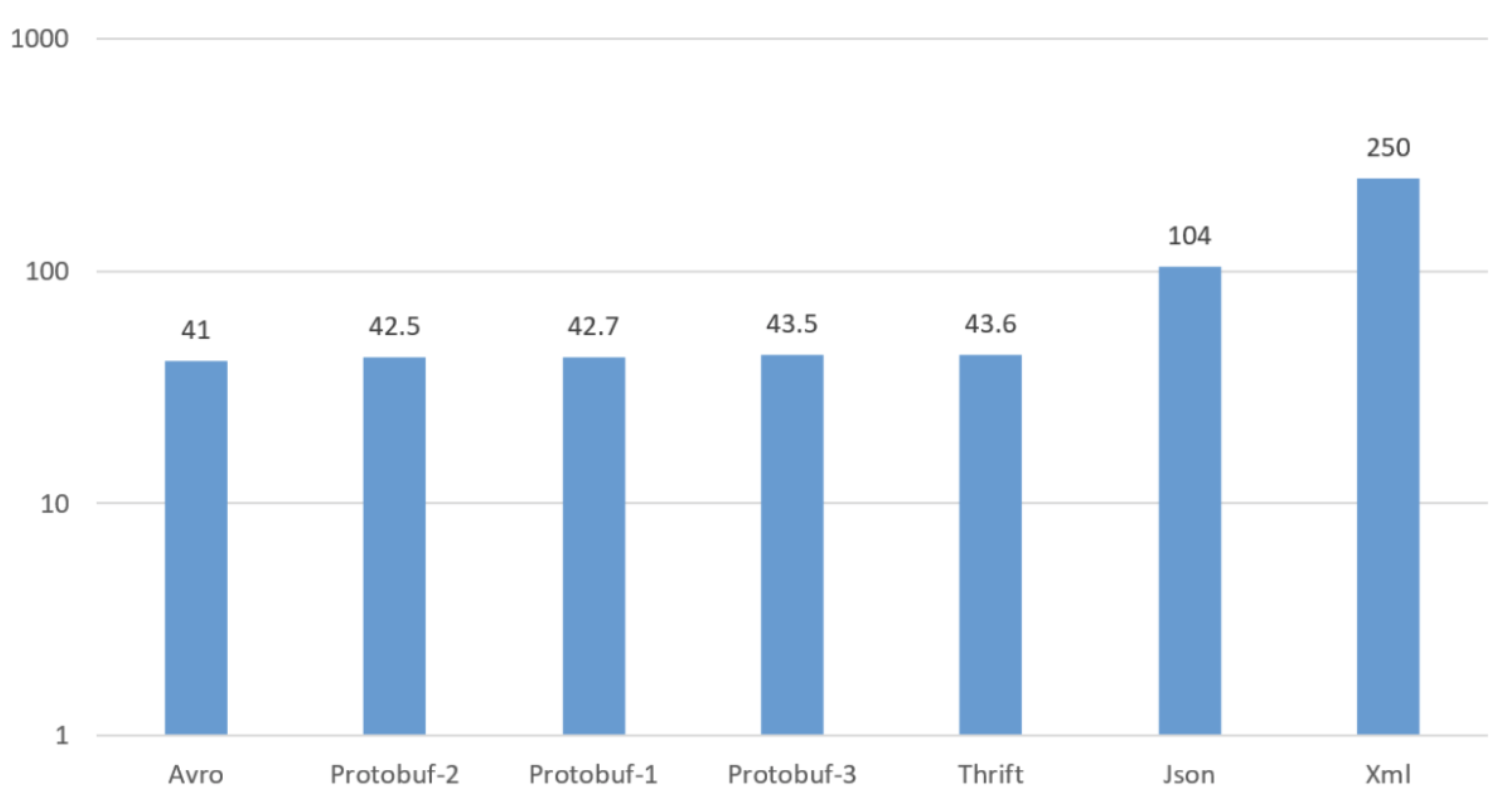
\includegraphics[width=15cm]{serialization_compression.png}
\end{figure}
\begin{figure}[H]
    \caption{Czasy serializacji i deserializacji w milisekundach}
    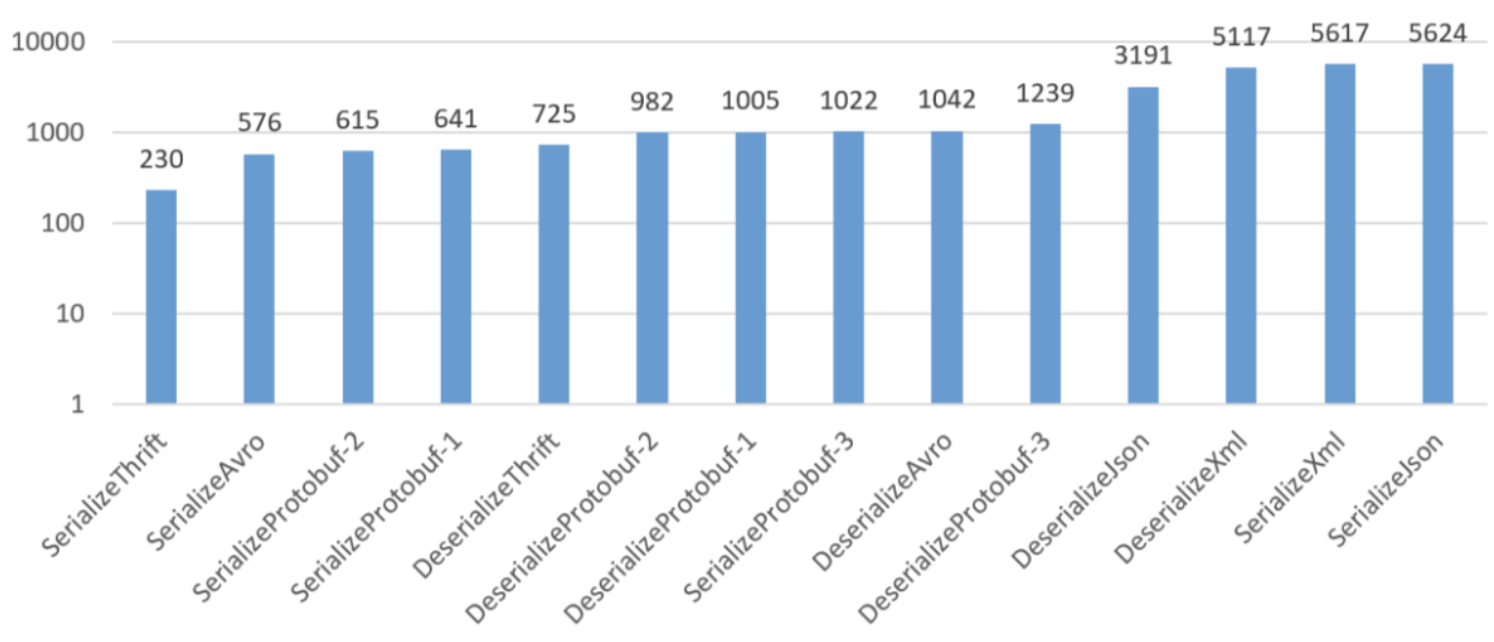
\includegraphics[width=15cm]{serialization_time.png}
\end{figure}

Z przedstawionych wykresów widać, że Avro, Protobuf i Thrift należą do czołówki serializatorów. W moim rozwiązaniu użyłem Avro, którego podstawowymi zaletami są \cite{avro, protobuf, thrift}:
\begin{itemize}
    \item szybkość zapisu i odczytu,
    \item kompresja danych do formatu binarnego,
    \item możliwość serializowania skomplikowanych obiektów,
    \item elastyczność schematów opisujących struktury serializowanych danych -- schematy zapisu i odczytu mogą być różne,
    \item klasa abstrakcyjna \textit{GenericData.Record} umożliwiająca generyczne operowanie na obiektach typu Avro.
\end{itemize}

Najważniejszy jest jednak fakt, że dzięki pakietowi Avro oraz możliwości dynamicznego tworzenia klas na podstawie schematów, biblioteka algorytmów minimalnych na Hadoopie jest generyczna. Każda funkcja i faza MapReduce może zostać zaaplikowana do dowolnego typu danych. Jest to ogromna zaleta biblioteki, ponieważ typowe programy MapReduce są pisane pod konkretne typy danych, a zmiana danych pociąga za sobą konieczność poprawiania programu.

\subsubsection{Zarządzanie maszynami} \label{hadoop_zarzadzanie_maszynami}

W przedstawionych algorytmach minimalnych można zauważyć jak ważna jest numeracja maszyn wchodzących w skład klastra. Niezwykle istotne jest utrzymywanie kolejności obiektów między maszynami. Dodatkowo fazy MapReduce wymagają wysyłania obiektów na konkretne maszyny. Także niektóre obliczenia wykonywane są tylko na wybranych maszynach.

Niestety Hadoop nie umożliwia ponumerowania lub oznaczania maszyn. Wszystkie maszyny oprócz \textit{NameNode} są równoważne i to YARN odpowiada za docelowe rozmieszczenie plików. Zaletą takiego rozwiązania jest fakt, że YARN wybierze maszyny, które są najbliżej danych i przesył informacji zostanie zoptymalizowany.

Rozwiązaniem, które zastosowałem jest wykorzystanie klucza, z pary wysyłanej przez MapReduce, jako numeru maszyny. Wszystkie fazy MapReduce zaimplementowane w bibliotece operują na parach \textit{<numerMaszyny, obiekty>}. Dzięki takiemu rozwiązaniu wszystkie obiekty, które powinny znaleźć się na maszynie \(M_i\), zostaną przetworzone przez jeden proces \textit{reduce}.

Niech \(i, j \in [0, \ liczbaMaszyn]\). W ramach biblioteki zostały zaimplementowane metody umożliwiające wysyłanie obiektów na:
\begin{itemize}
    \item konkretną maszynę \(i\),
    \item wszystkie maszyny w przedziale \([i, j)\),
    \item wszystkie maszyny większe niż \(i\),
    \item wszystkie maszyny mniejsze niż \(i\),
    \item wszystkie maszyny w systemie.
\end{itemize}

Funkcje zostały napisane w oparciu o klasy \textit{Mapper.Context} oraz \textit{Reducer.Context}, które są standardowym sposobem przesyłu niewielkich danych w Hadoopie.

\subsubsection{Przesył różnych typów obiektów} \label{hadoop_przesyl_obiektow}

Implementując niektóre algorytmy minimalne napotykamy problem jednoczesnego przesyłania różnych typów obiektów między fazami lub rundami MapReduce. Standardowo funkcje \textit{map} i \textit{reduce} pozwalają na przesył jednego typu elementów. Nie istnieje także klasa krotek działająca na obiektach generycznych.

W tym miejscu z pomocą przychodzi serializator Avro. Biblioteka algorytmów minimalnych implementuje klasę \textit{SendWrapper}, pozwalającą na wysyłanie zmieszanych typów danych. Na ten moment wspierana jest obsługa tylko dwóch typów obiektów. Rozszerzenie klasy na więcej typów jest jednak wykonalne i byłoby kompatybilne z obecną wersją biblioteki.

Klasa \textit{SendWrapper} opakowuje dwa obiekty Avro w jeden, tworząc schemat danych dynamicznie. Utworzony schemat posiada dwa opcjonalne pola. Gdy opakowujemy obiekt pierwszego typu, to drugie pole jest wartością \textit{null} i odwrotnie dla opakowywania elementu drugiego typu. Przesyłanie wartości \textit{null} jest niewielkim kosztem, który ponosimy za wspieranie funkcjonalności wysyłania dwóch typów obiektów. Dodatkowo biblioteka udostępnia funkcje pozwalające na filtrowanie elementów pierwszego / drugiego typu. Rysunek 4.3 przedstawia ogólną zasadę działania klasy \(SendWrapper\), a Listing \ref{hadoop_prefix} konkretny sposób zastosowania.

\begin{figure}[H]
    \caption{Przesyłanie dwóch typów obiektów}
    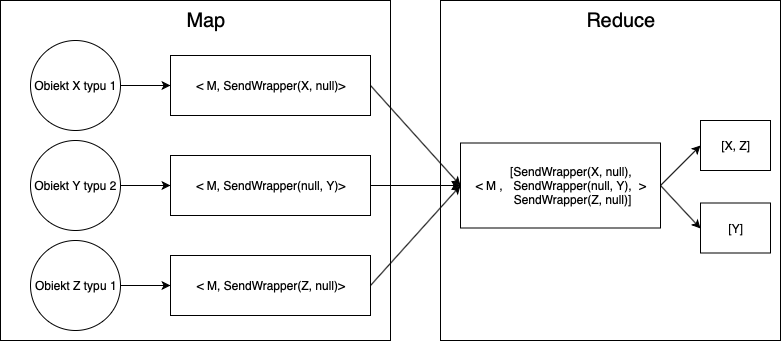
\includegraphics[width=15cm]{sending_multiple_typles.png}
\end{figure}

Alternatywą dla tego rozwiązania jest zapisywanie obiektów jednego z typów do plików na lokalnej pamięci maszyny, a następnie odczytywanie ich w fazie \(reduce\). Wadą takiego sposobu jest fakt, że rezygnujemy z automatycznego obsługiwania plików przez MapReduce oraz wykonujemy więcej operacji odczytu i zapisu.

Innym rozwiązaniem jest stworzenie dodatkowej rundy MapReduce, w której zapiszemy przetworzone obiekty do HDFS, a następnie odczytamy je w odpowiedniej fazie innej rundy algorytmu. Jest to rozwiązanie wolne i wymagające dodatkowej pracy.

\subsubsection{Statystyki} \label{hadoop_statystyki}

Kolejnym zagadnieniem jest implementacja funkcji statystyk łącznej na zdefiniowanym zbiorze obiektów. Rozwiązaniem, które zastosowałem jest stworzenie abstrakcyjnej klasy \mbox{\textit{StatisticsAggregator}} deklarującej dwie funkcje abstrakcyjne:
\begin{enumerate}
    \item \textit{public abstract void init(GenericRecord record)} - definiuje tworzenie statystyk na podstawie obiektu. Klasa \textit{GenericRecord} jest klasą abstrakcyją obiektów Avro.
    \item \textit{public abstract StatisticsAggregator merge(StatisticsAggregator that)} - opisuje sposób łączenia dwóch statystyk, \(stat(S) = merge(stat(S_1), stat(S_2))\), gdzie \(S_1\) i \(S_2\) tworzą podział \(S\), czyli \(S_1 \cup S_2 = S\) oraz \(S_1 \cap S_2 = \emptyset\).
\end{enumerate}

Użytkownik powinien stworzyć podklasę klasy \textit{StatisticsAggregator} i napisać definicje powyższych funkcji abstrakcyjnych. Proces implementacji składa się z następujących kroków i został przedstawiony na Listingach \ref{hadoop_avro_stats} oraz \ref{hadoop_stats_class}:
\begin{enumerate}
    \item Stworzenie schematu \textit{.avsc} dla klasy statystyk. Obiekty klasy statystyk są regularnymi obiektami, które są serializowalne i przesyłane między fazami MapReduce.
    \item Wygenerowanie klasy w Javie na podstawie pliku \textit{.avsc}.
    \item Zmodyfikowanie klasy utworzonej w kroku 2. Należy:
        \begin{itemize}
            \item podziedziczyć po klasie \textit{StatisticsAggregator},
            \item zaimplementować funkcje \textit{init} oraz \textit{merge}.
        \end{itemize}
\end{enumerate}

Zaletami takiego podejścia są:
\begin{itemize}
    \item definiowanie dowolnie skomplikowanych funkcji statystyk,
    \item obliczanie jednocześnie kilku funkcji statystyk przy jednej implementacji klasy reprezentującej statystyki,
    \item przechowywanie dodatkowych informacji związanych ze statystykami.
\end{itemize}

Biblioteka udostępnia także funkcje agregujące statystyki takie jak:
\begin{itemize}
    \item \textit{scanLeft} -- statystyki prefiksowe listy obiektów,
    \item \textit{foldLeft} -- agregacja statystyk z listy do pojedynczej wartości.
\end{itemize}

Dodatkowo została stworzona klasa \textit{RangeTree} umożliwiająca liczenie statystyk na przedziałach, w sposób sekwencyjny na pojedynczej maszynie. \textit{RangeTree} jest w pełni serializowalne co pozwala na przesyłanie uszeregowanych statystyk, a następnie wykonywanie optymalnych zapytań. Klasa implementuje klasyczne, pełne drzewo binarne oraz funkcje:
\begin{itemize}
    \item \textit{public void insert(StatisticsAggregator element, int pos)} -- wrzucanie statystyk do drzewa,
    \item \textit{public StatisticsAggregator query(int start, int end)} -- agregacja statystyk z zakresu \([start, end)\).
\end{itemize}

\subsubsection{Użytkowanie} \label{hadoop_uzytkowanie}

Pisanie programów na platformę Hadoop wymaga wiedzy i dokładności. Standardowo na początku użytkownik ustawia w konfiguracji programu wszelkie niezbędne parametry. Jednak system nie sprawdzana ich obecności i poprawności. Brak jednego z nich skutkuje zatrzymaniem wykonania programu i czasem straconym na znalezienie brakujących zmiennych.

W bibliotece algorytmów minimalnych wymagamy od użytkownika uzupełnienia wszystkich niezbędnych parametrów, a brak któregoś z nich jest sygnalizowany czytelnym komunikatem. Dodatkowo sprawdzana jest ich poprawność, aby uchronić użytkownika od banalnych błędów.

Biblioteka udostępnia także API do zarządzania plikami Avro na pamięci lokalnej maszyny. W jego skład wchodzą funkcje takie jak: \textit{zapis}, \textit{odczyt}, \textit{usuwanie}, ale także \textit{łączenie} dwóch plików Avro.

Dodatkowo istnieje funkcja, operująca na konfiguracji programu, zapisująca i odczytująca komparator obiektów Avro. Dzięki tej metodzie użytkownik raz zapisuje komparator do konfiguracji, a następnie może z niego korzystać w dowolnej fazie MapReduce.

\newpage
\section{Spark} \label{spark}

\subsection{Implementacja algorytmu bez użycia biblioteki} \label{sbub}
Na Listingu \ref{list_spark_run} przedstawiono implementację algorytmu statystyk prefiksowych bez użycia biblioteki. Dane wejściowe należały do klasy ukazanej na Listingu \ref{list_spark_four_ints}. Funkcję porównującą obiekty klasy \(FourInts\) przedstawiono na Listingu \ref{list_spark_cmp_four_ints}. Funkcją statystyk była suma wartości zwracanych przez funkcję \(getValue()\) -- Listing \ref{list_spark_four_ints}, linia 6.

\begin{lstlisting}[language=SmallJava,firstnumber=1,label=list_spark_four_ints,caption=Klasa danych wejściowych do algorytmu statystyk prefiksowych]
class FourInts(first: Int, second: Int, third: Int, fourth: Int) extends Serializable {
  def getFirst(): Int = this.first
  def getSecond(): Int = this.second
  def getThird(): Int = this.third
  def getFourth(): Int = this.fourth
  def getValue(): Int = this.getSecond() + this.getThird() + this.getFourth()
}
\end{lstlisting}

\begin{lstlisting}[language=SmallJava,firstnumber=1,label=list_spark_cmp_four_ints, caption=Funkcja porównująca obiekty klasy FourInts]
object FourInts {
  def cmpKey(o: FourInts): Int = o.getFirst()
}
\end{lstlisting}

Omówmy zwięźle Listing \ref{list_spark_run}. W liniach 6 -- 7 zaimplementowano algorytm \(TeraSort\), czyli rundy 1 -- 2 algorytmu statystyk prefiksowych. W tym celu użyto wbudowanej funkcji sortującej \textit{sortBy}. Następnie w liniach 9 -- 11 wykonujemy fazę \textit{map-shuffle}, polegającą na obliczeniu i rozesłaniu statystyk prefiksowych dla całych partycji. Funkcja \textit{partitionStatistics} iteruje po elementach RDD i wylicza sumę obiektów dla każdej partycji. Następnie \mbox{w linii 10} obliczamy sumy prefiksowe całych partycji, a w linii 11 rozsyłamy je na wszystkie maszyny. W~tym celu użyto wbudowanej funkcji \textit{broadcast}, która wysyła argument na każdą maszynę. Jest to wygodny sposób udostępniania obiektów innym partycjom, potrzebnych na wielu etapach obliczeń. Niestety postępując według algorytmu, powinniśmy rozsyłać statystyki prefiksowe partycji tylko do maszyn o większych indeksach. Zaimplementowana wersja algorytmu nie traci swojej minimalności, jednak jest wolniejsza i zużywa więcej pamięci. W~liniach \mbox{13 -- 24} wykonujemy fazę \textit{reduce}. Dzięki prostej funkcji statystyk oraz wcześniej udostępnionej liście \textit{distPartStats} w łatwy sposób obliczamy końcowy wynik algorytmu.
\newpage
\begin{lstlisting}[language=SmallJava,firstnumber=1,label=list_spark_run,caption=Implementacja algorytmu statystyk prefiksowych bez użycia biblioteki]
object PrefixApp {

  def prefix(sc: SparkContext, rdd: RDD[FourInts], numPartitions: Int):
        RDD[(Int, FourInts)] = {
    
    val sortedRdd = rdd.repartition(numPartitions).
        sortBy(FourInts.cmpKey).persist()

    val partStats = partitionStatistics(sortedRdd).collect()
    val prefixPartStats = partStats.scanLeft(0){(acc, o) => acc + o}
    val distPartStats = sc.broadcast(prefixPartStats).value

    sortedRdd.mapPartitionsWithIndex((pIndex, partitionIt) => {
      if (partitionIt.hasNext) {
        val elements = partitionIt.toList
        val prefixes = elements.scanLeft(distPartStats(pIndex)){
            (res, o) => res + o.getValue()
        }
        prefixes.zip(elements).iterator
      } else {
        Iterator()
      }
    })
  }

  def partitionStatistics(rdd: RDD[FourInts]): RDD[Int] = {
    rdd.mapPartitions(partitionIt => {
      if (partitionIt.isEmpty) {
        Iterator()
      } else {
        Iterator(partitionIt.foldLeft(0){(acc, o) => acc + o.getValue()})
      }
    })
  }
}
\end{lstlisting}

\subsection{Implementacja algorytmu z wykorzystaniem biblioteki}

Pisanie programów w Sparku jest łatwe i intuicyjne. Takie założenia spełnia też biblioteka do implementacji algorytmów minimalnych. Punktem wejściowym jest podanie dwóch argumentów (Listing \ref{list_spark_w_run}):
\begin{itemize}
    \item \textit{SparkSession} -- obiekt niezbędny do uruchomienia programu w Sparku,
    \item \textit{numberOfPartitions} -- liczba maszyn (partycji).
\end{itemize}

W przypadku algorytmów wymagających tylko posortowania, takich jak: \textit{TeraSort}, \textit{ranking}, \textit{pół-złączenia} użytkownik musi zdefiniować komparator obiektów wejściowych. Komparator jest pojedynczą funkcją, co pozwala na używanie wielu z nich przy raz wczytanych danych -- \mbox{linia 1, Listing \ref{list_spark_w_sum_agg}}.

Natomiast algorytmy agregujące statystyki, czyli: \textit{statystyki prefiksowe}, \textit{grupowanie}, \textit{statystyki okienkowe} wymuszają dodatkowe zaimplementowanie podklasy \textit{StatisticsAggregator} oraz zdefiniowanie funkcji \textit{init}, tak jak zostało to pokazane na Listingu \ref{list_spark_w_sum_agg}, odpowiednio linie 4 -- 12 oraz 2. Więcej informacji na temat obliczania statystyk w Sparku znajduje się w~podrozdziale \ref{spark_statystyki}.

\newpage
\begin{lstlisting}[language=SmallJava,firstnumber=1,label=list_spark_w_sum_agg,caption=Funkcja porównująca oraz funkcja statystyk]
val cmpKey = (o: FourInts) => o.getFirst
val sumAgg = (o: FourInts) => new SumAggregator(o.getValue)

class SumAggregator(value: Int)
    extends StatisticsAggregator[SumAggregator] {
    
  override def merge(that: SumAggregator): SumAggregator = {
    new SumAggregator(this.value + that.getValue)
  }
  
  def getValue: Int = value
}
\end{lstlisting}

Omówmy precyzyjniej Listing \ref{list_spark_w_run}. W liniach 4 -- 7 widzimy generyczną deklarację funkcji \(prefix\). Dzięki takiej formie, użytkownik może aplikować do funkcji dowolnie skomplikowane obiekty, które są porównywalne i posiadają funkcję zwracającą statystyki pojedynczego obiektu. W linii 9 sortujemy RDD za pomocą algorytmu \(TeraSort\), wykorzystującego wbudowaną w Sparka funkcję \(sortBy\).

Następnie w liniach 11 -- 12, dzięki wbudowanej w bibliotekę funkcji \(partitionStatistics\), obliczamy statystyki dla całych partycji. Wynik tych obliczeń łączymy z indeksami maszyn, które będą dolnymi ograniczeniami w przesyłaniu statystyk. Tak przygotowaną listę rozsyłamy do odpowiednich maszyn (linie 14 -- 15). Funkcja \( sendToAllHigherMachines\) jako argumenty przyjmuje obiekt \(SparkSession\), listę obiektów z dolnym ograniczeniem przesyłu oraz ilość wszystkich maszyn, czyli górne ograniczenie przesyłu. RDD \(distPartitionStatistics\) zawiera rozesłane statystki całych partycji zgodnie z opisem w podrozdziale \ref{statystyki_prefiksowe}, runda 3, faza \(map-shuffle\). Dokładne wyjaśnienie implementacji rozsyłania danych znajduje się w podrozdziale \ref{spark_zarzadzanie_maszynami}. Warto zauważyć, że pozbyliśmy się funkcji \(broadcast\) wykorzystanej na Listingu \ref{list_spark_run}, tym samym zoptymalizowaliśmy implementację algorytmu.

W ostatnim kroku, linie 17 -- 32, wykorzystujemy metodę \(zipPartitions\) w celu równoległego iterowania po posortowanych obiektach wejściowych oraz wcześniej rozesłanych statystykach całych partycji. Usunięcie funkcji \(broadcast\) zmusiło nas do iteracji po dwóch RDD zawierających różne typy danych. Jednak odpowiednia implementacja rozsyłania obiektów oraz wbudowana w Sparka metoda \(zipPartitions\) umożliwiają nam łatwe i efektywne implementowanie tej funkcjonalności. Dokładniejszy opis problemu i rozwiązania znajduje się w~podrozdziale \ref{spark_przesyl_obiektow}.

Do obliczenia wyniku dla każdego obiektu wykorzystujemy funkcje \(scanLeft\) oraz \(foldLeft\) z klasy \(StatisticsUtils\) wchodzącej w skład biblioteki. Ich użycie jest bardzo intuicyjne i przydatne w liczeniu generycznych, łącznych statystyk. Więcej na temat statystyk w~podrozdziale \ref{spark_statystyki}.

\newpage
\begin{lstlisting}[language=SmallJava,firstnumber=1,label=list_spark_w_run,caption=Implementacja algorytmu statystyk prefiksowych z wykorzystaniem biblioteki]
class MinimalAlgorithm(spark: SparkSession, numberOfPartitions: Int) {
  protected val sc: SparkContext = spark.sparkContext
  
  def prefix[T, K, S <: StatisticsAggregator[S]]
        (rdd: RDD[T], cmpKey: T => K, statsAgg: T => S)
        (implicit ord: Ordering[K], ttag: ClassTag[T],
         ktag: ClassTag[K], stag: ClassTag[S]): RDD[(S, T)] = {
         
    val sortedRdd = teraSort(rdd, cmpKey).persist()
    
    val partStatsWithBounds = StatisticsUtils.partitionStatistics(
        sortedRdd, statsAgg).collect().zip(List.range(0, numPartitions))
        
    val distPartitionStatistics = Utils.sendToAllHigherMachines(
        sc, partStatsWithBounds, numPartitions)
        
    sortedRdd.zipPartitions(distPartitionStatistics) {
        (partitionIt, partitionStatisticsIt) => {
      if (partitionIt.hasNext) {
        val elements = partitionIt.toList
        val statistics = elements.map{e => statsAgg(e)}
        val prefixes = if (partitionStatisticsIt.hasNext) {
          val startValue = StatisticsUtils.foldLeft(partitionStatisticsIt)
          StatisticsUtils.scanLeft(statistics, startValue).drop(1)
        } else {
          StatisticsUtils.scanLeft(statistics)
        }
        prefixes.zip(elements).iterator
      } else {
        Iterator()
      }
    }}
  }
}
\end{lstlisting}

Na podstawie Listingu \ref{list_spark_w_run} możemy stwierdzić, że implementacja generycznego algorytmu statystyk prefiksowych jest zwięzła i intuicyjna. Ilość kodu jest porównywalna do implementacji z Listingu \ref{list_spark_run}, jednak siła wyrazu Listingu \ref{list_spark_w_run} jest dużo większa. Użytkownik z łatwością może testować algorytm na różnych danych wejściowych, funkcjach statystyk czy komparatorach. Dodatkowo poprawiliśmy złożoność obliczeniową i pamięciową, rozsyłając statystyki prefiksowe maszyn tylko na wybrane partycje.

\subsection{Opis implementacji biblioteki}

Biblioteka jest oparta o wersję Spark 2.3 i jest napisana w języku Scala 2.11. Do zarządzania projektem użyto Apache Maven, programu automatyzującego budowę oprogramowania.

W podrozdziale \ref{sbub} zaobserwowaliśmy trudności związane z implementacją minimalnych algorytmów rozproszonych na Sparka. Głównymi z nich są:
\begin{itemize}
    \item brak precyzyjnego rozsyłania danych,
    \item słaba generyczności algorytmu.
\end{itemize}
W poniższych podrozdziałach przedstawię w jaki sposób biblioteka rozwiązuje powyższe problemy oraz pomaga implementować algorytmy minimalne.

\subsubsection{Zarządzanie maszynami} \label{spark_zarzadzanie_maszynami}

W Sparku nie możemy operować bezpośrednio na maszynach. Przykrywa je bowiem warstwa abstrakcji w postaci kolekcji rozproszonych danych, czyli RDD. Podstawową jednostką RDD są partycje. W moim rozwiązaniu to właśnie partycje symulują maszyny przedstawiane w algorytmach minimalnych.

RDD w API Sparka jest reprezentowane jako kolekcja partycji. Z tego wynika, że kolejne partycje mogą odpowiadać kolejnym maszynom. W mojej bibliotece wysyłanie obiektów na wybrane maszyny polega na zapisaniu ich na docelowych partycjach. Nie możemy jednak przesyłać pojedynczych elementów. Wszystkie operacje na RDD muszą być wykonywane przy pomocy transformacji. Rozwiązanie, które zaimplementowałem opiera się na przetasowywaniu RDD, a następnie jego podziale na partycje za pomocą zdefiniowanych podklas klasy \textit{Partitioner}. Biblioteka do implementacji algorytmów minimalnych zawiera dwie podklasy:
\begin{enumerate}
    \item \textit{KeyPartitioner} -- podział RDD wyznacza klucz obiektu, który jest docelowym indeksem maszyny,
    \item \textit{PerfectPartitioner} -- na podstawie rankingu obiektów dzieli RDD na partycje o równym rozmiarze, zgodnie z opisem w sekcji \ref{perfect_sort}.
\end{enumerate}

Powyższe rozwiązanie nie gwarantuje jednak zachowania kolejności elementów. RDD są stałe, czyli raz stworzone nie mogą ulec zmianie. Jednak nowe RDD są tworzone przez transformacje istniejących. Przekształcenia takie jak:
\begin{itemize}
    \item \textit{map} -- aplikowanie funkcji do obiektów na RDD,
    \item \textit{filter} -- filtrowanie obiektów RDD,
    \item \textit{mapPartitions} -- aplikowanie funkcji do całych partycji.
\end{itemize}
 
 utrzymują porządek na partycji. Natomiast istnieją też transformacje zaburzające kolejność elementów. Należą do nich między innymi:
 \begin{itemize}
     \item \textit{sortBy} -- sortowanie elementów,
     \item \textit{partitionBy} -- podział RDD na nowe partycje za pomocą zdefiniowanej klasy podziału.
 \end{itemize}

W przypadku wysyłania obiektów na wszystkie maszyny, została zaimplementowana też druga, konkurencyjna metoda. Wykorzystuje ona metodę \textit{broadcast}. Polega na natychmiastowym stworzeniu stałej, zapisanej w pamięci podręcznej każdego węzła klastra. Spark optymalizuje wysyłanie takich zmiennych, zatem jest to dobra opcja do przesłania kopii dużych zbiorów danych potrzebnych na wielu etapach obliczeń. W sytuacji, gdy kopie wszystkich elementów są potrzebne tylko w następnej transformacji, lepiej użyć leniwie wykonującego się \textit{Partitionera} z pierwszego rozwiązania \cite{spark_documentation}.

Tak jak w przypadku Hadoopa, udostępnione zostały następujące funkcje przesyłu obiektów na:
\begin{itemize}
    \item konkretną maszynę \(i\),
    \item wszystkie maszyny w przedziale \([i, j)\),
    \item wszystkie maszyny większe niż \(i\),
    \item wszystkie maszyny mniejsze niż \(i\),
    \item wszystkie maszyny w systemie,
\end{itemize}

gdzie \(i, j \in [0, \ liczbaMaszyn]\).

\subsubsection{Przesył różnych typów obiektów} \label{spark_przesyl_obiektow}

Na platformie Spark również doświadczamy problemu przesyłania różnych typów obiektów między transformacjami RDD. W tej sekcji przedstawię możliwe rozwiązania tego problemu oraz uargumentuję wybór zaimplementowanej metody.

Pierwszym ze sposobów jest użycie metody \textit{broadcast}. Jak już wspomniałem wcześniej, jest to dobre rozwiązanie, gdy chcemy używać przesyłanych obiektów na wszystkich maszynach i w dodatku w kilku transformacjach. W przeciwnym przypadku marnujemy tylko zasoby Sparka.

Inną możliwością jest wykorzystanie klasy \textit{Accumulator} udostępnianej przez Sparka. Obiekty tej klasy są współdzielonymi akumulatorami, do których można dodawać obiekty tylko podczas przemiennej, asocjacyjnej transformacji np: \textit{map}. Co więcej, węzły wykonawcze (\textit{DataNode}) mogą tylko zapisywać dane, a jedynie węzeł główny (\textit{NameNode}) może je odczytywać \cite{spark_documentation}. Niestety oba powyższe fakty znacząco ograniczają możliwości użycia akumulatorów.

Kolejnym rozwiązaniem jest zapisywanie obiektów do rozproszonego systemu danych np: HDFS. Jednak w Sparku byłoby to ogromne spowolnienie dla całego programu. Standardowo zapis danych do pamięci następuje tylko w momencie utrwalenia ostatecznych rezultatów lub gdy brakuje pamięci operacyjnej \cite{zaharia2010spark}.

Następnym sposobem jest rozwiązanie podobne do zaimplementowanego w bibliotece algorytmów minimalnych na Hadoopa. Sprowadza się ono do mieszania obiektów różnych typów na jednym RDD. Rozwiązanie wykorzystywałoby API Sparka, dzięki czemu byłoby łatwe w obsłudze i bardziej efektywne niż zapis do rozproszonego systemu danych. Niestety w momencie transformacji wymagałoby rozdzielenia obiektów, co generowałoby dodatkowe koszty czasowe.

Ostatnim i wybranym rozwiązaniem jest łączenie RDD. API Sparka udostępnia metodę \mbox{\textit{zipPartitions}} pozwalającą na równoległe iterowanie po od dwóch do czterech RDD, zachowując przy tym kolejność partycji i obiektów. RDD muszą składać się z takiej samej liczby partycji. W momencie równoległego iterowania, partycje zostaną połączone w takiej kolejności, w jakiej występują na danym RDD. Zaimplementowanie równoległego przesyłu różnych typów obiektów składa się z następujących kroków:
\begin{enumerate}
    \item Wysyłamy obiekty typu \textbf{I} na wybrane maszyny $\rightarrow$ powstaje nowe \(Rdd1\) -- na \mbox{Listingu \ref{list_spark_w_run}} jest nim \(sortedRDD\),
    \item Wysyłamy obiekty typu \textbf{II} na wybrane maszyny $\rightarrow$ powstaje nowe \(Rdd2\) -- na \mbox{Listingu \ref{list_spark_w_run}} jest nim \(distPartitionStatistics\),
    \item Łączymy \textit{Rdd1} z \textit{Rdd2} i aplikujemy transformację:
    $$Rdd1.zipPartitions(Rdd2)\{(partitions1Iter, \ partitions2Iter) => \{ ... \}\}$$
    
    Za pomocą iteratorów \(partitions1Iter\) oraz \(partitions2Iter\) mamy dostęp do obiektów z partycji odpowiednio Rdd1 i Rdd2. Przykład użycia przedstawiono na Listingu \ref{list_spark_w_run} linie 19 -- 31.
\end{enumerate}

\newpage
\subsubsection{Statystyki} \label{spark_statystyki}

Problem liczenia statystyk na Sparku rozwiązałem w sposób bardzo podobny do tego na Hadoopie. Została stworzona klasa abstrakcyjna \textit{StatisticsAggregator} deklarująca funkcję abstrakcyjną
$$def \ merge(statisticsAggregator: S): S $$ gdzie \textit{S} jest podklasą klasy \textit{StatisticsAggregator}. Funkcja \textit{merge}, tak samo jak w Hadoopie, definiuje proces łączenia dwóch statystyk. Po stronie użytkownika pozostaje stworzenie klasy \textit{S} oraz zdefiniowanie funkcji $init: T \rightarrow S$, gdzie \textit{T} jest typem obiektów wejściowych. Na Listingu \ref{list_spark_w_sum_agg} znajduje się przykład implementacji takiej klasy statystyk (linie 4 -- 12) oraz funkcji \(init\) (linia 2). Definiowanie funkcji \textit{init} poza klasą \textit{S} umożliwia większą elastyczność i generalizację w użytkowaniu i pisaniu algorytmów.

Biblioteka do implementacji algorytmów minimalnych udostępnia także następujące operacje na statystykach:
\begin{itemize}
    \item \textit{scanLeft} -- statystyki prefiksowe dla kolekcji,
    \item \textit{foldLeft} -- agregacja statystyk z kolekcji do pojedynczej wartości,
    \item \textit{scanLeftPartitions} -- statystyki prefiksowe na partycjach zawartych w RDD,
    \item \textit{partitionStatistics} -- statystyki dla każdej partycji zawartej w RDD.
\end{itemize}

Identycznie jak w rozwiązaniu na Hadoopa, została zaimplementowana klasa \textit{RangeTree}, umożliwiająca liczenie statystyk na przedziałach, w sposób sekwencyjny na pojedynczej maszynie. Klasa implementuje klasyczne, pełne drzewo binarne oraz funkcje:
\begin{itemize}
    \item \textit{insert(element: StatisticsAggregator, position: Int): Unit} -- wrzucanie statystyk do drzewa,
    \item \textit{query(start: Int, end: Int): StatisticsAggregator} -- agregacja statystyk z zakresu \([start, end)\).
\end{itemize}

\chapter{Testy}

Biblioteka do implementacji algorytmów minimalnych zawiera zestaw testów poprawnościowych sprawdzających działanie metod API i przykładowych algorytmów minimalnych w spreparowanym środowisku oraz skrypty testujące ich efektywność w warunkach produkcyjnych. Dodatkowo w ramach pracy przeprowadziłem testy wydajnościowe na zaimplementowanych algorytmach. Przy użyciu generatora losowych danych typu Avro (https://github.com/confluentinc/avro-random-generator) stworzyłem dwie grupy danych ważące 1 GB (10 000 000 obiektów) i 5 GB (45 000 000 obiektów). Obiekty zostały stworzone przy pomocy  schematu z Listingu \ref{list_test_schema}:

\begin{lstlisting}[language=SmallJava,firstnumber=1,label=list_test_schema,caption=Schemat obiektów użytych podczas testowania]
{ "type": "record",
  "name": "Complex",
  "namespace": "complex.type",
  "fields":
    [
      { "name": "null_prim", "type": ["null", "int"] },
      { "name": "boolean_prim", "type": "boolean" },
      { "name": "int_prim", "type": {
          "type": "int",
          "arg.properties": {
            "range": {
              "min": -10,
              "max": 10
            }
          }
        }
      },
      { "name": "long_prim", "type": "long" },
      { "name": "float_prim", "type": "float" },
      { "name": "double_prim", "type": "double" },
      { "name": "string_prim", "type": "string" },
      { "name": "bytes_prim", "type": "bytes" },
      { "name": "middle", "type":
        { "type": "record",
          "name": "MiddleNested",
          "fields": [
            { "name": "middle_array",
              "type": {
                "type": "array",
                "items": "float"
              }
            },
            { "name": "inner",
              "type": {
                "type": "record",
                "name": "InnerNested",
                "fields": [
                  { "name": "inner_int",
                    "type": "int"
                  },
                  { "name": "inner_string",
                    "type": "string"
                  }
                ]
              }
            }
          ]
        }
      }
    ]
}
\end{lstlisting}

Testy zostały przeprowadzone na dwóch typach klastrów składających się z:
\begin{itemize}
    \item 1 NameNode + 5 DataNode
    \item 1 NameNode + 10 DataNode
\end{itemize}

Klastry zostały utworzone na platformie \textit{Amazon Web Services}. Każdy NameNode \mbox{i DataNode} posiadał 4-rdzeniowy procesor oraz 6 GB pamięci RAM. Do porównywania obiektów został wykorzystany komparator z Listingu \ref{list_test_cmp}:
\begin{lstlisting}[language=SmallJava,firstnumber=1,label=list_test_cmp,caption=Komparator obiektów użyty podczas testowania]
public class ComplexComparator implements Comparator<Complex> {
    @Override
    public int compare(Complex o1, Complex o2) {
        int innerInt1 = o1.getMiddle().getInner().getInnerInt();
        int innerInt2 = o2.getMiddle().getInner().getInnerInt();
        return innerInt1 > innerInt2 ?
            1 : (innerInt1 < innerInt2 ?
                -1 : o1.getLongPrim() > o2.getLongPrim() ?
                    1 : o1.getLongPrim() < o2.getLongPrim() ?
                        -1 : 0));
    }
}
\end{lstlisting}

\section{Hadoop}
\setlength{\parindent}{6.5ex}
W poniższych sekcjach zostały przedstawione wyniki testów poszczególnych algorytmów minimalnych wykonanych na Hadoopie. Kolumny mają następujące znaczenie:
\begin{itemize}
    \item Runda -- runda algorytmu MapReduce opisana w sekcji \ref{algorytmy_minimalne},
    \item Czas (s) -- całkowity czas wykonania algorytmu,
    \item Max zużycie pamięci (GB) -- maksymalne zużycie pamięci na całym klastrze podczas wykonywania algorytmu,
    \item Max przesył danych (GB) -- maksymalny przesył danych wewnątrz całego klastra podczas wykonywania algorytmu.
\end{itemize}

\subsection{TeraSort}

\begin{table}[H]
\centering
\caption{Wykonanie algorytmu \textit{TeraSort}}
\label{tab:my-table}
\resizebox{\textwidth}{!}{%
\begin{tabular}{@{}cccccc@{}}
\toprule
Wielkość danych (GB) & Liczba maszyn & Runda       & Czas (s) & Max zużycie pamięci (GB) & Max przesył danych (GB) \\ \midrule
                     &              & Próbkowanie & 43       & 4,785                    & 0,003                   \\
1                    & 5            & Sortowanie  & 104      & 12,062                   & 1,187                   \\ \midrule
                     &              & Próbkowanie & 83       & 20,252                   & 0,005                   \\
5                    & 5            & Sortowanie  & 273      & 34,677                   & 5,099                   \\ \midrule
                     &              & Próbkowanie & 41       & 4,643                    & 0,003                   \\
1                    & 10           & Sortowanie  & 70       & 12,303                   & 1,133                   \\ \midrule
                     &              & Próbkowanie & 55       & 19,612                   & 0,012                   \\
5                    & 10           & Sortowanie  & 139      & 40,187                   & 5,101                   \\ \bottomrule
\end{tabular}%
}
\end{table}

\subsection{Lista rankingowa}

\begin{table}[H]
\centering
\caption{Wykonanie algorytmu \textit{lista rankingowa}}
\label{tab:my-table}
\resizebox{\textwidth}{!}{%
\begin{tabular}{@{}cccccc@{}}
\toprule
Wielkość danych (GB) & Liczba maszyn & Runda       & Czas (s) & Max zużycie pamięci (GB) & Max przesył danych (GB) \\ \midrule
                     &              & Próbkowanie & 43       & 4,575                    & 0,003                   \\
1                    & 5            & Sortowanie  & 101      & 11,011                   & 1,137                   \\
                     &              & Ranking     & 77       & 13,197                   & 1,094                   \\ \midrule
                     &              & Próbkowanie & 81       & 20,452                   & 0,005                   \\
5                    & 5            & Sortowanie  & 267      & 34,687                   & 5,109                   \\
                     &              & Ranking     & 226      & 36,123                   & 4,923                   \\ \midrule
                     &              & Próbkowanie & 40       & 4,653                    & 0,003                   \\
1                    & 10           & Sortowanie  & 71       & 12,203                   & 1,123                   \\
                     &              & Ranking     & 66       & 15,865                   & 1,094                   \\ \midrule
                     &              & Próbkowanie & 53       & 19,312                   & 0,012                   \\
5                    & 10           & Sortowanie  & 138      & 39,587                   & 5,081                   \\
                     &              & Ranking     & 120      & 38,440                   & 4,923                   \\ \bottomrule
\end{tabular}%
}
\end{table}

\subsection{Statystyki prefiksowe}

W algorytmie statystyk prefiksowych użyto sumy jako funkcji statystyk.

\begin{table}[H]
\centering
\caption{Wykonanie algorytmu \textit{statystyki prefiksowe}}
\label{tab:my-table}
\resizebox{\textwidth}{!}{%
\begin{tabular}{@{}cccccc@{}}
\toprule
Wielkość danych (GB) & Liczba maszyn & Runda       & Czas (s) & Max zużycie pamięci (GB) & Max przesył danych (GB) \\ \midrule
                     &              & Próbkowanie & 41       & 4,575                    & 0,003                   \\
1                    & 5            & Sortowanie  & 102      & 11,021                   & 1,137                   \\
                     &              & Prefix      & 95       & 13,326                   & 1,148                   \\ \midrule
                     &              & Próbkowanie & 80       & 20,552                   & 0,005                   \\
5                    & 5            & Sortowanie  & 266      & 34,667                   & 5,106                   \\
                     &              & Prefix      & 255      & 32,260                   & 5,185                   \\ \midrule
                     &              & Próbkowanie & 41       & 4,643                    & 0,003                   \\
1                    & 10           & Sortowanie  & 70       & 12,213                   & 1,133                   \\
                     &              & Prefix      & 85       & 16,017                   & 1,148                   \\ \midrule
                     &              & Próbkowanie & 53       & 19,312                   & 0,012                   \\
5                    & 10           & Sortowanie  & 138      & 39,587                   & 5,081                   \\
                     &              & Prefix      & 140      & 42,469                   & 5,185                   \\ \bottomrule
\end{tabular}%
}
\end{table}

\subsection{Grupowanie}

W algorytmie grupowania użyto sumy jako funkcji statystyk.

\begin{table}[H]
\centering
\caption{Wykonanie algorytmu \textit{grupowania}}
\label{tab:my-table}
\resizebox{\textwidth}{!}{%
\begin{tabular}{@{}cccccc@{}}
\toprule
Wielkość danych (GB) & Liczba maszyn & Runda       & Czas (s) & Max zużycie pamięci (GB) & Max przesył danych (GB) \\ \midrule
                     &              & Próbkowanie & 41       & 4,555                    & 0,003                   \\
1                    & 5            & Sortowanie  & 101      & 11,011                   & 1,117                   \\
                     &              & Grupowanie  & 49       & 8,899                    & 0,0001                  \\ \midrule
                     &              & Próbkowanie & 79       & 20,532                   & 0,005                   \\
5                    & 5            & Sortowanie  & 265      & 34,657                   & 5,101                   \\
                     &              & Grupowanie  & 126      & 27,279                   & 0,0006                  \\ \midrule
                     &              & Próbkowanie & 40       & 4,623                    & 0,003                   \\
1                    & 10           & Sortowanie  & 71       & 12,211                   & 1,113                   \\
                     &              & Grupowanie  & 51       & 10,842                   & 0,0001                  \\ \midrule
                     &              & Próbkowanie & 52       & 19,311                   & 0,011                   \\
5                    & 10           & Sortowanie  & 137      & 39,567                   & 5,071                   \\
                     &              & Grupowanie  & 80       & 30,526                   & 0,0001                  \\ \bottomrule
\end{tabular}%
}
\end{table}

\subsection{Statystyka okienkowa}
W algorytmie statystyki okienkowej użyto sumy jako funkcji statystyk.

\begin{table}[H]
\centering
\caption{Wykonanie algorytmu \textit{statystyki okienkowej}}
\label{tab:my-table}
\resizebox{\textwidth}{!}{%
\begin{tabular}{@{}cccccc@{}}
\toprule
Wielkość danych (GB) & Liczba maszyn & Runda                  & Czas (s) & Max zużycie pamięci (GB) & Max przesył danych (GB) \\ \midrule
                     &              & Próbkowanie            & 40       & 4,556                    & 0,003                   \\
                     &              & Sortowanie             & 102      & 11,012                   & 1,116                   \\
1                    & 5            & Ranking                & 86       & 13,198                   & 1,093                   \\
                     &              & Perf. sortowanie & 94       & 13,994                   & 1,168                   \\
                     &              & Stat. okienkowa    & 141      & 16,168                   & 2,366                   \\ \midrule
                     &              & Próbkowanie            & 78       & 20,531                   & 0,005                   \\
                     &              & Sortowanie             & 261      & 34,655                   & 5,101                   \\
5                    & 5            & Ranking                & 198      & 32,732                   & 4,923                   \\
                     &              & Perf. sortowanie & 257      & 40,410                   & 5,255                   \\
                     &              & Stat. okienkowa    & 473      & 36,515                   & 10,703                  \\ \midrule
                     &              & Próbkowanie            & 41       & 4,623                    & 0,003                   \\
                     &              & Sortowanie             & 71       & 12,211                   & 1,113                   \\
1                    & 10           & Ranking                & 68       & 16,429                   & 1,094                   \\
                     &              & Perf. sortowanie & 82       & 17,788                   & 1,168                   \\
                     &              & Stat. okienkowa    & 103      & 24,364                   & 2,366                   \\ \midrule
                     &              & Próbkowanie            & 52       & 19,311                   & 0,011                   \\
                     &              & Sortowanie             & 137      & 39,567                   & 5,071                   \\
5                    & 10           & Ranking                & 126      & 40,335                   & 4,922                   \\
                     &              & Perf. sortowanie & 155      & 46,564                   & 5,254                   \\
                     &              & Stat. okienkowa    & 276      & 44,522                   & 10,629                  \\ \bottomrule
\end{tabular}%
}
\end{table}

\subsection{Podsumowanie}

\begin{table}[H]
\centering
\caption{Podsumowanie wykonania algorytmu \textit{TeraSort} na Hadoopie.}
\label{tab:my-table}
\resizebox{\textwidth}{!}{%
\begin{tabular}{@{}ccccc@{}}
\toprule
Wielkość danych (GB) & Liczba maszyn & Czas (s) & Max zużycie pamięci (GB) & Max przesył danych (GB) \\ \midrule
1                    & 5            & 152      & 12,062                   & 1,187                   \\ \midrule
5                    & 5            & 364      & 34,677                   & 5,099                   \\ \midrule
1                    & 10           & 116      & 12,303                   & 1,133                   \\ \midrule
5                    & 10           & 199      & 40,187                   & 5,101                  
\\ \bottomrule
\end{tabular}%
}
\end{table}

\begin{table}[H]
\centering
\caption{Podsumowanie wykonania algorytmu \textit{listy rankingowej} na Hadoopie.}
\label{tab:my-table}
\resizebox{\textwidth}{!}{%
\begin{tabular}{@{}ccccc@{}}
\toprule
Wielkość danych (GB) & Liczba maszyn & Czas (s) & Max zużycie pamięci (GB) & Max przesył danych (GB) \\ \midrule
1                    & 5            & 231      & 13,197                   & 1,137                   \\ \midrule
5                    & 5            & 584      & 36,123                   & 5,109                   \\ \midrule
1                    & 10           & 187      & 15,865                   & 1,123                   \\ \midrule
5                    & 10           & 321      & 39,587                   & 5,081                   \\ \bottomrule
\end{tabular}%
}
\end{table}

\begin{table}[H]
\centering
\caption{Podsumowanie wykonania algorytmu \textit{statystyk prefiksowych} na Hadoopie.}
\label{tab:my-table}
\resizebox{\textwidth}{!}{%
\begin{tabular}{@{}ccccc@{}}
\toprule
Wielkość danych (GB) & Liczba maszyn & Czas (s) & Max zużycie pamięci (GB) & Max przesył danych (GB) \\ \midrule
1                    & 5            & 248      & 13,326                   & 1,148                   \\ \midrule
5                    & 5            & 611      & 34,667                   & 5,185                   \\ \midrule
1                    & 10           & 206      & 16,017                   & 1,148                   \\ \midrule
5                    & 10           & 341      & 42,469                   & 5,185                   \\ \bottomrule
\end{tabular}%
}
\end{table}

\begin{table}[H]
\centering
\caption{Podsumowanie wykonania algorytmu \textit{grupowania} na Hadoopie.}
\label{tab:my-table}
\resizebox{\textwidth}{!}{%
\begin{tabular}{@{}ccccc@{}}
\toprule
Wielkość danych (GB) & Liczba maszyn & Czas (s) & Max zużycie pamięci (GB) & Max przesył danych (GB) \\ \midrule
1                    & 5            & 201      & 11,011                   & 1,117                   \\ \midrule
5                    & 5            & 480      & 34,657                   & 5,101                   \\ \midrule
1                    & 10           & 172      & 12,211                   & 1,113                   \\ \midrule
5                    & 10           & 279      & 39,567                   & 5,071                   \\ \bottomrule
\end{tabular}%
}
\end{table}

\begin{table}[H]
\centering
\caption{Podsumowanie wykonania algorytmu \textit{statystyk okienkowych} na Hadoopie.}
\label{tab:my-table}
\resizebox{\textwidth}{!}{%
\begin{tabular}{@{}ccccc@{}}
\toprule
Wielkość danych (GB) & Liczba maszyn & Czas (s) & Max zużycie pamięci (GB) & Max przesył danych (GB) \\ \midrule
1                    & 5            & 473      & 16,168                   & 2,366                   \\ \midrule
5                    & 5            & 1277     & 40,410                   & 10,703                  \\ \midrule
1                    & 10           & 375      & 24,364                   & 2,366                   \\ \midrule
5                    & 10           & 756      & 46,564                   & 10,629                  \\ \bottomrule
\end{tabular}%
}
\end{table}

Algorytmy \textit{TeraSort}, \textit{lista rankingowa}, \textit{statystyki prefiksowe} oraz \textit{grupowanie} mają bardzo zbliżone maksymalne zużycie pamięci oraz maksymalny przesył danych. Jedynie algorytm \textit{statystyki okienkowej} zużywa więcej pamięci oraz transferu danych. Wynika to z faktu replikowania obiektów w ostatniej rundzie algorytmu.

Wszystkie algorytmy zakończyły się w skończonej liczbie rund (3 lub 5). Wbudowane narzędzie do monitorowania rund MapReduce nie obejmuje statystyk dotyczących zużytej pamięci i transferu danych na poszczególnych maszynach. Widać jednak, że maksymalne zużycie pamięci oraz maksymalny przesył danych na całym klastrze są ograniczone przez liczbę obiektów wejściowych. Dodatkowo czas, pamięć i transfer spadają liniowo wraz ze wzrostem ilości maszyn oraz wzrastają liniowo wraz ze wzrostem wielkości danych wejściowych. Na tej podstawie można stwierdzić, że implementacje przykładowych algorytmów minimalnych na Hadoopa przy użyciu biblioteki spełniają założenia klasy algorytmów minimalnych.

\section{Spark}

W podrozdziale zostały przedstawione wyniki testów poszczególnych algorytmów minimalnych zaimplementowanych przy użyciu biblioteki i uruchomionych na Sparku. Kolumny mają następujące znaczenie:
\begin{itemize}
    \item Wielkość danych (GB) -- wielkość danych wejściowych,
    \item Liczba maszyn -- liczba maszyn DataNode użytych do wykonania algorytmu,
    \item Min / Max / Średni czas (s) -- minimalny / maksymalny / średni czas wykonania rundy algorytmu na maszynie,
    \item Min / Max / Średnia pamięć (GB) -- minimalne / maksymalne / średnie zużycie pamięci na maszynie,
    \item Min / Max / Średni przesył danych (GB) -- minimalny / maksymalny / średni przesył danych na maszynie.
\end{itemize}

\subsection{TeraSort}

\begin{table}[H]
\centering
\caption{Wykonanie algorytmu \textit{TeraSort} na Sparku.}
\label{tab:my-table}
\resizebox{\textwidth}{!}{%
\begin{tabular}{cccccccccccc}
\toprule
\begin{tabular}[c]{@{}c@{}}Wielkość\\ danych\\ (GB)\end{tabular} & \begin{tabular}[c]{@{}c@{}}Liczba\\ maszyn\end{tabular} & Runda      & \begin{tabular}[c]{@{}c@{}}Min\\ czas\\ (s)\end{tabular} & \begin{tabular}[c]{@{}c@{}}Max\\ czas\\ (s)\end{tabular} & \begin{tabular}[c]{@{}c@{}}Średni\\ czas\\ (s)\end{tabular} & \begin{tabular}[c]{@{}c@{}}Min\\ pamięć\\ (GB)\end{tabular} & \begin{tabular}[c]{@{}c@{}}Max\\ pamięć\\ (GB)\end{tabular} & \begin{tabular}[c]{@{}c@{}}Średnia\\ pamięć\\ (GB)\end{tabular} & \begin{tabular}[c]{@{}c@{}}Min\\ przesył\\ danych\\ (GB)\end{tabular} & \begin{tabular}[c]{@{}c@{}}Max\\ przesył\\ danych\\  (GB)\end{tabular} & \begin{tabular}[c]{@{}c@{}}Średni\\ przesył\\ danych\\ (GB)\end{tabular} \\ \midrule
1                                                              & 5                                                      & Sortowanie & 14                                                     & 17                                                     & 16                                                        & 0,221                                                     & 0,225                                                     & 0,224                                                         & 0                                                                 & 0                                                                  & 0                                                                    \\ \hline
5                                                              & 5                                                      & Sortowanie & 24                                                     & 26                                                     & 25                                                        & 0,944                                                     & 1,002                                                     & 1,001                                                         & 0                                                                 & 0                                                                  & 0                                                                    \\ \hline
1                                                              & 10                                                     & Sortowanie & 11                                                     & 15                                                     & 13                                                        & 0,108                                                     & 0,112                                                     & 0,112                                                         & 0                                                                 & 0                                                                  & 0                                                                    \\ \hline
5                                                              & 10                                                     & Sortowanie & 26                                                     & 30                                                     & 28                                                        & 0,500                                                     & 0,504                                                     & 0,504                                                         & 0                                                                 & 0                                                                  & 0                                                                    \\ \hline
\end{tabular}%
}
\end{table}

\subsection{Lista rankingowa}

\begin{table}[H]
\large
\centering
\caption{Wykonanie algorytmu \textit{lista rankingowa} na Sparku.}
\label{tab:my-table}
\resizebox{\textwidth}{!}{%
\begin{tabular}{@{}cccccccccccc@{}}
\toprule
\begin{tabular}[c]{@{}c@{}}Wielkość\\ danych\\ (GB)\end{tabular} & \begin{tabular}[c]{@{}c@{}}Liczba\\ maszyn\end{tabular} & Runda      & \begin{tabular}[c]{@{}c@{}}Min\\ czas\\ (s)\end{tabular} & \begin{tabular}[c]{@{}c@{}}Max\\ czas\\ (s)\end{tabular} & \begin{tabular}[c]{@{}c@{}}Średni\\ czas\\ (s)\end{tabular} & \begin{tabular}[c]{@{}c@{}}Min\\ pamięć\\ (GB)\end{tabular} & \begin{tabular}[c]{@{}c@{}}Max\\ pamięć\\ (GB)\end{tabular} & \begin{tabular}[c]{@{}c@{}}Średnia\\ pamięć\\ (GB)\end{tabular} & \begin{tabular}[c]{@{}c@{}}Min\\ przesył\\ danych\\ (GB)\end{tabular} & \begin{tabular}[c]{@{}c@{}}Max\\ przesył\\ danych\\  (GB)\end{tabular} & \begin{tabular}[c]{@{}c@{}}Średni\\ przesył\\ danych\\ (GB)\end{tabular} \\ \midrule
                                                                &                                                         & Sortowanie & 14                                                      & 17                                                      & 16                                                         & 0,221                                                      & 0,225                                                      & 0,224                                                          & 0,000                                                              & 0,000                                                               & 0,000                                                                  \\
1                                                               & 5                                                       & Ranking    & 117                                                     & 160                                                     & 133                                                        & 3,800                                                      & 5,100                                                      & 4,240                                                          & 0,357                                                              & 0,460                                                               & 0,392                                                                  \\ \midrule
                                                                &                                                         & Sortowanie & 24                                                      & 25                                                      & 25                                                         & 0,943                                                      & 1,002                                                      & 1,001                                                          & 0,000                                                              & 0,000                                                               & 0,000                                                                  \\
5                                                               & 5                                                       & Ranking    & 720                                                     & 740                                                     & 733                                                        & 18,600                                                     & 20,500                                                     & 19,840                                                         & 1,671                                                              & 1,849                                                               & 1,760                                                                  \\ \midrule
                                                                &                                                         & Sortowanie & 11                                                      & 15                                                      & 13                                                         & 0,108                                                      & 0,113                                                      & 0,112                                                          & 0,000                                                              & 0,000                                                               & 0,000                                                                  \\
1                                                               & 10                                                      & Ranking    & 70                                                      & 85                                                      & 78                                                         & 1,671                                                      & 1,676                                                      & 1,673                                                          & 0,172                                                              & 0,212                                                               & 0,195                                                                  \\ \midrule
                                                                &                                                         & Sortowanie & 26                                                      & 30                                                      & 28                                                         & 0,500                                                      & 0,505                                                      & 0,504                                                          & 0,000                                                              & 0,000                                                               & 0,000                                                                  \\
5                                                               & 10                                                      & Ranking    & 280                                                     & 315                                                     & 302                                                        & 9,000                                                      & 10,600                                                     & 9,890                                                          & 0,815                                                              & 0,950                                                               & 0,882                                                                  \\ \bottomrule
\end{tabular}%
}
\end{table}

\subsection{Statystyki prefiksowe}

W algorytmie statystyk prefiksowych użyto sumy jako funkcji statystyk.

\begin{table}[H]
\centering
\caption{Wykonanie algorytmu \textit{statystyki prefiksowe} na Sparku.}
\label{tab:my-table}
\resizebox{\textwidth}{!}{%
\begin{tabular}{@{}cccccccccccc@{}}
\toprule
\begin{tabular}[c]{@{}c@{}}Wielkość\\ danych\\ (GB)\end{tabular} & \begin{tabular}[c]{@{}c@{}}Liczba\\ maszyn\end{tabular} & Runda      & \begin{tabular}[c]{@{}c@{}}Min\\ czas\\ (s)\end{tabular} & \begin{tabular}[c]{@{}c@{}}Max\\ czas\\ (s)\end{tabular} & \begin{tabular}[c]{@{}c@{}}Średni\\ czas\\ (s)\end{tabular} & \begin{tabular}[c]{@{}c@{}}Min\\ pamięć\\ (GB)\end{tabular} & \begin{tabular}[c]{@{}c@{}}Max\\ pamięć\\ (GB)\end{tabular} & \begin{tabular}[c]{@{}c@{}}Średnia\\ pamięć\\ (GB)\end{tabular} & \begin{tabular}[c]{@{}c@{}}Min\\ przesył\\ danych\\ (GB)\end{tabular} & \begin{tabular}[c]{@{}c@{}}Max\\ przesył\\ danych\\  (GB)\end{tabular} & \begin{tabular}[c]{@{}c@{}}Średni\\ przesył\\ danych\\ (GB)\end{tabular} \\ \midrule
                                                                &                                                         & Sortowanie & 15                                                      & 17                                                      & 16                                                         & 0,221                                                      & 0,226                                                      & 0,224                                                          & 0,000                                                              & 0,000                                                               & 0,000                                                                 \\
1                                                               & 5                                                       & Prefix     & 125                                                     & 157                                                     & 138                                                        & 3,400                                                      & 5,100                                                      & 4,240                                                          & 0,337                                                              & 0,443                                                               & 0,390                                                                 \\ \midrule
                                                                &                                                         & Sortowanie & 24                                                      & 25                                                      & 25                                                         & 0,954                                                      & 1,002                                                      & 1,001                                                          & 0,000                                                              & 0,000                                                               & 0,000                                                                 \\
5                                                               & 5                                                       & Prefix     & 720                                                     & 740                                                     & 733                                                        & 18,800                                                     & 20,700                                                     & 19,940                                                         & 1,632                                                              & 1,832                                                               & 1,760                                                                 \\ \midrule
                                                                &                                                         & Sortowanie & 11                                                      & 14                                                      & 12                                                         & 0,108                                                      & 0,112                                                      & 0,112                                                          & 0,000                                                              & 0,000                                                               & 0,000                                                                 \\
1                                                               & 10                                                      & Prefix     & 70                                                      & 77                                                      & 74                                                         & 1,661                                                      & 1,673                                                      & 1,668                                                          & 0,174                                                              & 0,212                                                               & 0,195                                                                 \\ \midrule
                                                                &                                                         & Sortowanie & 24                                                      & 25                                                      & 24                                                         & 0,500                                                      & 0,504                                                      & 0,504                                                          & 0,000                                                              & 0,000                                                               & 0,000                                                                 \\
5                                                               & 10                                                      & Prefix     & 285                                                     & 335                                                     & 309                                                        & 9,000                                                      & 10,600                                                     & 9,880                                                          & 0,815                                                              & 0,950                                                               & 0,882                                                                 \\ \bottomrule
\end{tabular}%
}
\end{table}

\newpage
\subsection{Grupowanie}

W algorytmie grupowania użyto sumy jako funkcji statystyk.

\begin{table}[H]
\centering
\caption{Wykonanie algorytmu \textit{grupowania} na Sparku.}
\label{tab:my-table}
\resizebox{\textwidth}{!}{%
\begin{tabular}{@{}cccccccccccc@{}}
\toprule
\begin{tabular}[c]{@{}c@{}}Wielkość\\ danych\\ (GB)\end{tabular} & \begin{tabular}[c]{@{}c@{}}Liczba\\ maszyn\end{tabular} & Runda      & \begin{tabular}[c]{@{}c@{}}Min\\ czas\\ (s)\end{tabular} & \begin{tabular}[c]{@{}c@{}}Max\\ czas\\ (s)\end{tabular} & \begin{tabular}[c]{@{}c@{}}Średni\\ czas\\ (s)\end{tabular} & \begin{tabular}[c]{@{}c@{}}Min\\ pamięć\\ (GB)\end{tabular} & \begin{tabular}[c]{@{}c@{}}Max\\ pamięć\\ (GB)\end{tabular} & \begin{tabular}[c]{@{}c@{}}Średnia\\ pamięć\\ (GB)\end{tabular} & \begin{tabular}[c]{@{}c@{}}Min\\ przesył\\ danych\\ (GB)\end{tabular} & \begin{tabular}[c]{@{}c@{}}Max\\ przesył\\ danych\\  (GB)\end{tabular} & \begin{tabular}[c]{@{}c@{}}Średni\\ przesył\\ danych\\ (GB)\end{tabular} \\ \midrule
                                                                &                                                         & Sortowanie & 15                                                      & 17                                                      & 16                                                         & 0,221                                                      & 0,225                                                      & 0,224                                                          & 0,000                                                              & 0,000                                                               & 0,000                                                                  \\
1                                                               & 5                                                       & Grupowanie & 65                                                      & 85                                                      & 75                                                         & 3,100                                                      & 5,500                                                      & 4,200                                                          & 0,274                                                              & 0,470                                                               & 0,372                                                                  \\ \midrule
                                                                &                                                         & Sortowanie & 24                                                      & 26                                                      & 25                                                         & 0,944                                                      & 1,002                                                      & 1,001                                                          & 0,000                                                              & 0,000                                                               & 0,000                                                                  \\
5                                                               & 5                                                       & Grupowanie & 275                                                     & 375                                                     & 353                                                        & 19,600                                                     & 20,000                                                     & 19,740                                                         & 1,648                                                              & 1,649                                                               & 1,648                                                                  \\ \midrule
                                                                &                                                         & Sortowanie & 11                                                      & 15                                                      & 13                                                         & 0,108                                                      & 0,112                                                      & 0,112                                                          & 0,000                                                              & 0,000                                                               & 0,000                                                                  \\
1                                                               & 10                                                      & Grupowanie & 39                                                      & 42                                                      & 41                                                         & 1,662                                                      & 1,668                                                      & 1,664                                                          & 0,183                                                              & 0,184                                                               & 0,183                                                                  \\ \midrule
                                                                &                                                         & Sortowanie & 25                                                      & 30                                                      & 28                                                         & 0,502                                                      & 0,503                                                      & 0,505                                                          & 0,000                                                              & 0,000                                                               & 0,000                                                                  \\
5                                                               & 10                                                      & Grupowanie & 171                                                     & 186                                                     & 177                                                        & 11,400                                                     & 11,400                                                     & 11,400                                                         & 0,824                                                              & 0,825                                                               & 0,824                                                                  \\ \bottomrule
\end{tabular}%
}
\end{table}

\subsection{Statystyki okienkowe}

W algorytmie statystyk okienkowych użyto sumy jako funkcji statystyk.

\begin{table}[H]
\centering
\caption{Wykonanie algorytmu \textit{statystyk okienkowych} na Sparku.}
\label{tab:my-table}
\resizebox{\textwidth}{!}{%
\begin{tabular}{@{}cccccccccccc@{}}
\toprule
\begin{tabular}[c]{@{}c@{}}Wielkość\\ danych\\ (GB)\end{tabular} & \begin{tabular}[c]{@{}c@{}}Liczba\\ maszyn\end{tabular} & Runda      & \begin{tabular}[c]{@{}c@{}}Min\\ czas\\ (s)\end{tabular} & \begin{tabular}[c]{@{}c@{}}Max\\ czas\\ (s)\end{tabular} & \begin{tabular}[c]{@{}c@{}}Średni\\ czas\\ (s)\end{tabular} & \begin{tabular}[c]{@{}c@{}}Min\\ pamięć\\ (GB)\end{tabular} & \begin{tabular}[c]{@{}c@{}}Max\\ pamięć\\ (GB)\end{tabular} & \begin{tabular}[c]{@{}c@{}}Średnia\\ pamięć\\ (GB)\end{tabular} & \begin{tabular}[c]{@{}c@{}}Min\\ przesył\\ danych\\ (GB)\end{tabular} & \begin{tabular}[c]{@{}c@{}}Max\\ przesył\\ danych\\  (GB)\end{tabular} & \begin{tabular}[c]{@{}c@{}}Średni\\ przesył\\ danych\\ (GB)\end{tabular} \\ \midrule
                                                               &                                                        & Sortowanie    & 15                                                     & 17                                                     & 16                                                        & 0,221                                                     & 0,225                                                      & 0,224                                                         & 0,000                                                              & 0,000                                                               & 0,000                                                                 \\
1                                                              & 5                                                      & Ranking    & 124                                                    & 158                                                    & 136                                                       & 3,800                                                     & 5,100                                                      & 4,300                                                         & 0,377                                                              & 0,453                                                               & 0,411                                                                 \\
                                                               &                                                        & Perf. sortowanie    & 164                                                    & 196                                                    & 179                                                       & 3,700                                                     & 4,800                                                      & 4,400                                                         & 0,365                                                              & 0,431                                                               & 0,387                                                                 \\
                                                               &                                                        & Stat. okienkowa    & 64                                                     & 68                                                     & 65                                                        & 3,500                                                     & 3,500                                                      & 3,500                                                         & 0,726                                                              & 0,726                                                               & 0,726                                                                 \\ \midrule
                                                               &                                                        & Sortowanie    & 23                                                     & 25                                                     & 24                                                        & 0,945                                                     & 1,001                                                      & 0,999                                                         & 0,000                                                              & 0,000                                                               & 0,000                                                                 \\
5                                                              & 10                                                     & Ranking    & 310                                                    & 342                                                    & 331                                                       & 19,000                                                    & 20,800                                                     & 20,100                                                        & 2,800                                                              & 3,100                                                               & 2,900                                                                 \\
                                                               &                                                        & Perf. sortowanie    & 439                                                    & 470                                                    & 455                                                       & 23,300                                                    & 26,800                                                     & 24,800                                                        & 3,500                                                              & 3,700                                                               & 3,700                                                                 \\
                                                               &                                                        & Stat. okienkowa    & 198                                                    & 223                                                    & 212                                                       & 22,300                                                    & 24,700                                                     & 23,500                                                        & 1,600                                                              & 1,700                                                               & 1,700                                                                 \\ \midrule
                                                               &                                                        & Sortowanie    & 11                                                     & 15                                                     & 13                                                        & 0,108                                                     & 0,111                                                      & 0,112                                                         & 0,000                                                              & 0,000                                                               & 0,000                                                                 \\
1                                                              & 10                                                     & Ranking    & 75                                                     & 85                                                     & 81                                                        & 1,672                                                     & 1,672                                                      & 1,672                                                         & 0,188                                                              & 0,204                                                               & 0,199                                                                 \\
                                                               &                                                        & Perf. sortowanie    & 82                                                     & 93                                                     & 88                                                        & 1,672                                                     & 1,801                                                      & 1,701                                                         & 0,365                                                              & 0,383                                                               & 0,377                                                                 \\
                                                               &                                                        & Stat. okienkowa    & 48                                                     & 50                                                     & 49                                                        & 3,400                                                     & 3,500                                                      & 3,500                                                         & 0,362                                                              & 0,362                                                               & 0,362                                                                 \\ \midrule
                                                               &                                                        & Sortowanie    & 25                                                     & 30                                                     & 28                                                        & 0,501                                                     & 0,504                                                      & 0,503                                                         & 0,000                                                              & 0,000                                                               & 0,000                                                                 \\
5                                                              & 10                                                     & Ranking    & 246                                                    & 253                                                    & 248                                                       & 10,400                                                    & 10,700                                                     & 10,500                                                        & 1,500                                                              & 1,600                                                               & 1,500                                                                 \\
                                                               &                                                        & Perf. sortowanie    & 280                                                    & 294                                                    & 288                                                       & 11,500                                                    & 11,700                                                     & 11,600                                                        & 1,800                                                              & 1,900                                                               & 1,800                                                                 \\
                                                               &                                                        & Stat. okienkowa    & 112                                                    & 123                                                    & 115                                                       & 14,300                                                    & 14,500                                                     & 14,400                                                        & 2,600                                                              & 2,700                                                               & 2,700                                                                 \\ \bottomrule
\end{tabular}%
}
\end{table}

\subsection{Podsumowanie}

\begin{table}[H]
\centering
\caption{Podsumowanie algorytmu \textit{TeraSort} przy użyciu Sparka.}
\label{tab:my-table}
\resizebox{\textwidth}{!}{%
\begin{tabular}{@{}ccccc@{}}
\toprule
\begin{tabular}[c]{@{}c@{}}Wielkość\\ danych (GB)\end{tabular} & Liczba maszyn & Czas (s) & \begin{tabular}[c]{@{}c@{}}Max zużycie pamięci\\ na poj. maszynie (GB)\end{tabular} & \begin{tabular}[c]{@{}c@{}}Max przesył danych\\ na poj. maszynie (GB)\end{tabular} \\ \midrule
1                                                              & 5            & 41       & 0,225                                                                               & 0                                                                                  \\ \midrule
5                                                              & 5            & 66       & 1,002                                                                               & 0                                                                                  \\ \midrule
1                                                              & 10           & 37       & 0,112                                                                               & 0                                                                                  \\ \midrule
5                                                              & 10           & 52       & 0,504                                                                               & 0                                                                                  \\ \bottomrule
\end{tabular}%
}
\end{table}

\begin{table}[H]
\centering
\caption{Podsumowanie algorytmu \textit{lista rankingowa} na Sparku.}
\label{tab:my-table}
\resizebox{\textwidth}{!}{%
\begin{tabular}{@{}ccccc@{}}
\toprule
\begin{tabular}[c]{@{}c@{}}Wielkość\\ danych (GB)\end{tabular} & Liczba maszyn & Czas (s) & \begin{tabular}[c]{@{}c@{}}Max zużycie pamięci\\ na poj. maszynie (GB)\end{tabular} & \begin{tabular}[c]{@{}c@{}}Max przesył danych\\ na poj. maszynie (GB)\end{tabular} \\ \midrule
1                                                              & 5            & 192      & 5,100                                                                               & 0,460                                                                              \\ \midrule
5                                                              & 5            & 780      & 20,500                                                                              & 1,849                                                                              \\ \midrule
1                                                              & 10           & 115      & 1,676                                                                               & 0,212                                                                              \\ \midrule
5                                                              & 10           & 360      & 10,600                                                                              & 0,950                                                                              \\ \bottomrule
\end{tabular}%
}
\end{table}

\begin{table}[H]
\centering
\caption{Podsumowanie algorytmu \textit{statystyki prefiksowe} na Sparku.}
\label{tab:my-table}
\resizebox{\textwidth}{!}{%
\begin{tabular}{@{}ccccc@{}}
\toprule
\begin{tabular}[c]{@{}c@{}}Wielkość\\ danych (GB)\end{tabular} & Liczba maszyn & Czas (s) & \begin{tabular}[c]{@{}c@{}}Max zużycie pamięci\\ na poj. maszynie (GB)\end{tabular} & \begin{tabular}[c]{@{}c@{}}Max przesył danych\\ na poj. maszynie (GB)\end{tabular} \\ \midrule
1                                                              & 5            & 189      & 5,100                                                                               & 0,443                                                                              \\ \midrule
5                                                              & 5            & 780      & 20,700                                                                              & 1,832                                                                              \\ \midrule
1                                                              & 10           & 106      & 1,673                                                                               & 0,212                                                                              \\ \midrule
5                                                              & 10           & 375      & 10,600                                                                              & 0,950                                                                              \\ \bottomrule
\end{tabular}%
}
\end{table}

\begin{table}[H]
\centering
\caption{Podsumowanie algorytmu \textit{grupowania} na Sparku.}
\label{tab:my-table}
\resizebox{\textwidth}{!}{%
\begin{tabular}{@{}ccccc@{}}
\toprule
\begin{tabular}[c]{@{}c@{}}Wielkość\\ danych (GB)\end{tabular} & Liczba maszyn & Czas (s) & \begin{tabular}[c]{@{}c@{}}Max zużycie pamięci\\ na poj. maszynie (GB)\end{tabular} & \begin{tabular}[c]{@{}c@{}}Max przesył danych\\ na poj. maszynie (GB)\end{tabular} \\ \midrule
1                                                              & 5            & 117      & 5,500                                                                               & 0,470                                                                              \\ \midrule
5                                                              & 5            & 416      & 20,000                                                                              & 1,649                                                                              \\ \midrule
1                                                              & 10           & 72       & 1,668                                                                               & 0,184                                                                              \\ \midrule
5                                                              & 10           & 231      & 11,400                                                                              & 0,825                                                                              \\ \bottomrule
\end{tabular}%
}
\end{table}

\begin{table}[H]
\centering
\caption{Podsumowanie algorytmu \textit{statystyk okienkowych} na Sparku.}
\label{tab:my-table}
\resizebox{\textwidth}{!}{%
\begin{tabular}{@{}ccccc@{}}
\toprule
\begin{tabular}[c]{@{}c@{}}Wielkość\\ danych (GB)\end{tabular} & Liczba maszyn & Czas (s) & \begin{tabular}[c]{@{}c@{}}Max zużycie pamięci\\ na poj. maszynie (GB)\end{tabular} & \begin{tabular}[c]{@{}c@{}}Max przesył danych\\ na poj. maszynie (GB)\end{tabular} \\ \midrule
1                                                              & 5            & 454      & 5,100                                                                               & 0,726                                                                              \\ \midrule
5                                                              & 5            & 1075     & 26,800                                                                              & 3,700                                                                              \\ \midrule
1                                                              & 10           & 258      & 3,500                                                                               & 0,383                                                                              \\ \midrule
5                                                              & 10           & 715      & 14,500                                                                              & 2,700                                                                              \\ \bottomrule
\end{tabular}%
}
\end{table}

Algorytmy \textit{lista rankingowa}, \textit{statystyki prefiksowe} oraz \textit{grupowanie} mają bardzo zbliżone maksymalne zużycie pamięci oraz maksymalny przesył danych. Algorytm \textit{statystyk okienkowych}, na tle pozostałych algorytmów, zużywa więcej pamięci oraz transferu danych. Wynika to z~faktu replikowania obiektów w ostatniej rundzie algorytmu.

Statystyki algorytmu \textit{TeraSort} znacząco odstają od wyników reszty algorytmów. W~bibliotece do implementacji algorytmów minimalnych został użyty wbudowany w Sparka algorytm sortowania i w związku z tym jest bardzo dobrze zoptymalizowany. Dodatkowo składa się z jednej rundy. Pozostałe algorytmy minimalne korzystają z wyniku sortowania i muszą zapisać go w pamięci RAM. Niestety maszyny wchodzące w skład klastra posiadały tylko 6 GB pamięci RAM i w związku z tym pomiędzy kolejnymi rundami algorytmu zapisywały dane do pamięci lokalnej maszyny. Skutkowało to zwiększeniem zużytej pamięci, a także wydłużeniem czasu wykonania.

Wszystkie algorytmy zakończyły się w skończonej liczbie rund. Maksymalne zużycie pamięci oraz maksymalny przesył danych są ograniczone przez liczbę obiektów wejściowych. Dodatkowo czas, pamięć i transfer spadają liniowo wraz ze wzrostem ilości maszyn oraz wzrastają liniowo wraz ze wzrostem wielkości danych wejściowych.

Warto także zauważyć, że wartości minimalne i maksymalne w obrębie czasów wykonania, zużycia pamięci oraz transferu danych nie są od siebie bardzo oddalone, co świadczy o~równomiernym obciążeniu maszyn.

Na podstawie powyższych statystyk i analiz można stwierdzić, że implementacje przedstawionych algorytmów minimalnych na Sparka przy użyciu biblioteki spełniają założenia klasy algorytmów minimalnych.

\newpage
\section{Porównanie Hadoop vs Spark}

W podrozdziale porównano statystyki wykonania na Sparku i Hadoopie przykładowych algorytmów minimalnych zaimplementowanych przy użyciu biblioteki.

\begin{figure}[H]
\centering
  \caption{Porównanie czasów wykonania algorytmów minimalnych na 1 GB danych przy użyciu 5 maszyn.}
  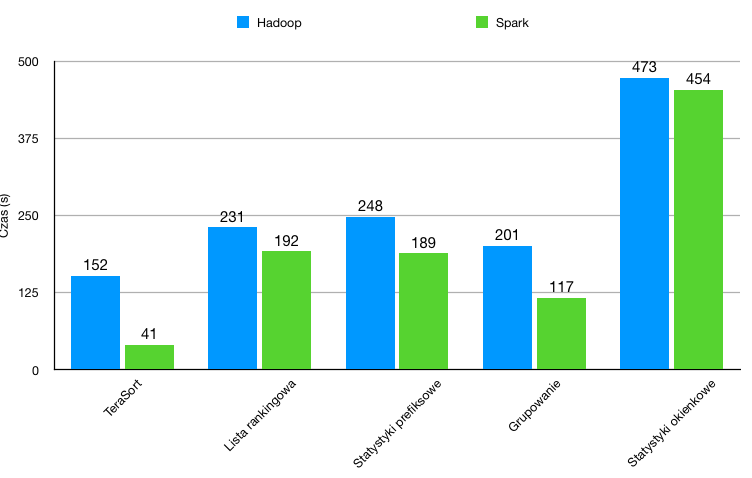
\includegraphics[width=13cm]{1_5_execution.png}
\end{figure}

\begin{figure}[H]
\centering
  \caption{Porównanie czasów wykonania algorytmów minimalnych na 5 GB danych przy użyciu 5 maszyn.}
  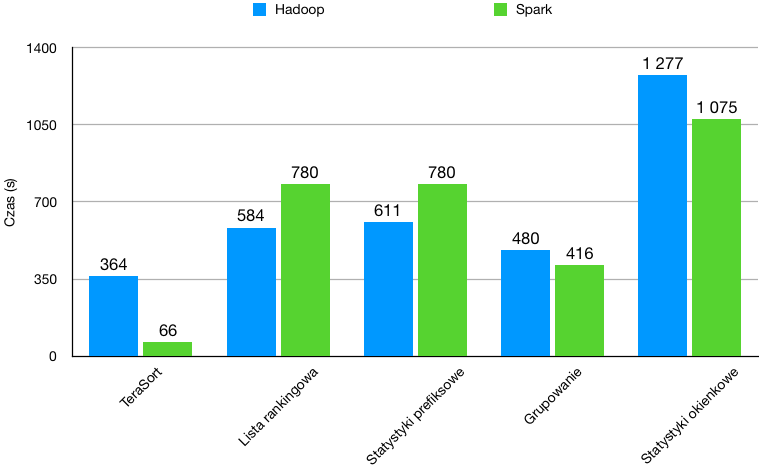
\includegraphics[width=13cm]{5_5_execution.png}
\end{figure}

\begin{figure}[H]
\centering
  \caption{Porównanie czasów wykonania algorytmów minimalnych na 1 GB danych przy użyciu 10 maszyn.}
  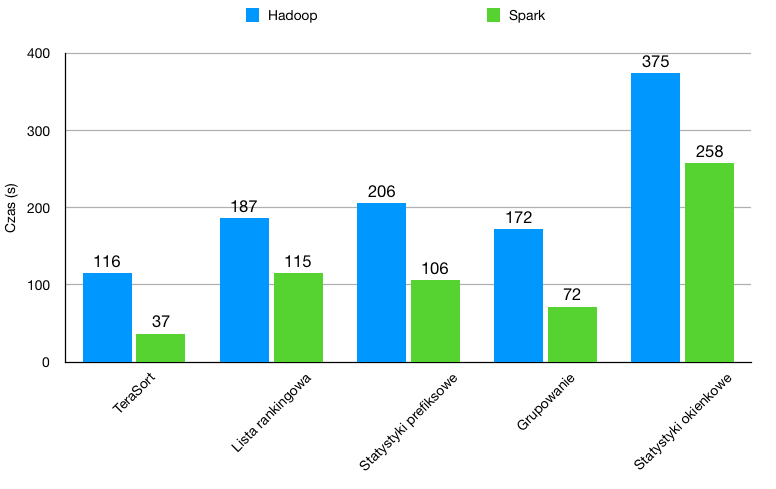
\includegraphics[width=13cm]{1_10_execution.png}
\end{figure}

\begin{figure}[H]
\centering
  \caption{Porównanie czasów wykonania algorytmów minimalnych na 5 GB danych przy użyciu 10 maszyn.}
  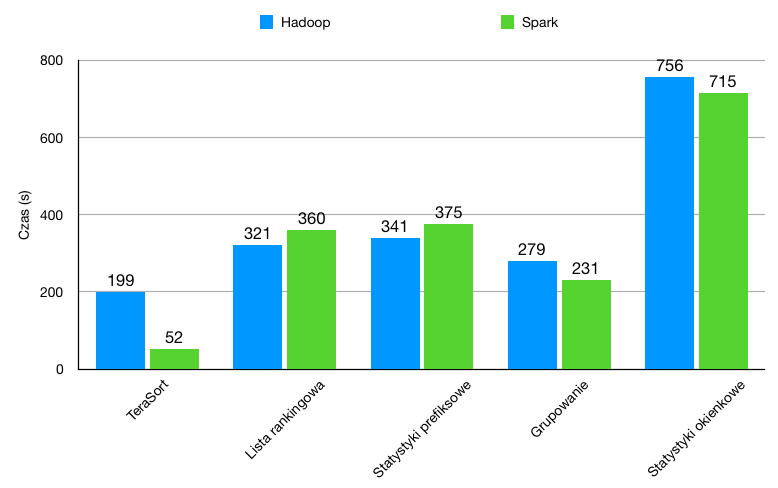
\includegraphics[width=13cm]{5_10_execution.png}
\end{figure}

\newpage
Z wykresów na Rysunkach 5.1, 5.2, 5.3 oraz 5.4 wynika, że algorytm \textit{TeraSort} jest znacząco szybszy na Sparku. W implementacji Sparka \textit{grupowanie} oraz \textit{statystyka okienkowa} są zawsze szybsze, jednak \textit{lista rankingowa} oraz \textit{statystyki prefiksowe} niekoniecznie. Możemy zauważyć, że wielkość danych wejściowych odgrywa bardzo ważną rolę. Przy rozmiarze danych \mbox{1 GB} wszystkie algorytmy na Sparku są znacząco szybsze niż na Hadoopie. Natomiast przy wielkości danych 5 GB różnica maleje, a w przypadku \textit{listy rankingowej} oraz \textit{statystyk prefiksowych} Hadoop wygrywa. Powodem takiego zachowania jest zbyt mała ilość pamięci RAM na maszynach wchodzących w skład klastra. Jak wcześniej było wspomniane, Spark zawdzięcza swoją szybkość operacjom \textit{in-memory}. Niestety w przypadku zbyt małej ilości pamięci RAM, ta przewaga zostaje zniwelowana, a dodatkowo system musi zapisywać i odczytywać dane z~dysku, tym samym tracąc swoją najcenniejszą właściwość.

\chapter{Podsumowanie}
\setlength{\parindent}{6.5ex}

Biblioteka do implementacji algorytmów minimalnych powstała z myślą ułatwienia i przyspieszenia procesu tworzenia nowych algorytmów minimalnych oraz szybkiego dostępu do istniejących implementacji. W obecnych czasach programowanie rozproszone jest coraz powszechniej stosowane i dlatego uważam, że biblioteka idealnie wpasowuje się w aktualny trend pracy nad efektywnym przetwarzaniem ogromnych zbiorów informacji.

Obie biblioteki udostępniają szereg funkcjonalności takich jak wysyłanie obiektów na konkretne maszyny, równoległe operowanie na różnych typach danych oraz funkcje do obliczania łącznych statystyk na zbiorach.

Implementacja na Hadoopa wydaje się być dobrym narzędziem do używania, tworzenia i rozwijania algorytmów minimalnych. Posiada zwięzłe API oraz ułatwia korzystanie z paradygmatu MapReduce. Umożliwia także pisanie generycznych algorytmów MapReduce. Testy przykładowych algorytmów minimalnych wypadły bardzo obiecująco. Niepokojące może być wysokie zużycie pamięci lokalnej maszyn. W przyszłości warto by powtórzyć testy, mierząc statystyki oddzielnie dla każdej maszyny wchodzącej w skład klastra. Dodatkowo warto przeprowadzić testy w warunkach identycznych do opisanych w pracy \cite{tao2013minimal}, a następnie porównać wyniki.

Rozwiązanie na Sparka, pod kątem łatwości użytkowania wypada bardzo dobrze. Biblioteka jest intuicyjna w użyciu i komponuje się ze stylem programowania na Sparka. Oprócz wcześniej wymienionych funkcjonalności, umożliwia także pisanie generycznych algorytmów rozproszonych. Niestety w aspekcie efektywności, implementacja na Sparka prezentuje się nieco gorzej niż na Hadoopa. Z testów przeprowadzonych na przykładowych algorytmach minimalnych można wyciągnąć wniosek, że biblioteka nie jest do końca zoptymalizowana. Potwierdza to brak zdecydowanej przewagi Sparka nad Hadoopem pod względem efektywności. Dodatkowo fakt, że algorytm \textit{TeraSort} zaimplementowany przy użyciu wbudowanego w~Sparka algorytmu sortowania ma dużo lepsze statystyki niż reszta przykładowych algorytmów, pokazuje że biblioteka może zostać zoptymalizowana. Warto spojrzeć na \(lineage\) i uważnie przyjrzeć się kolejnym etapom wykonania algorytmu. Należałoby także powtórzyć testy na klastrze złożonym z maszyn o większej ilości pamięci RAM.

Obecna wersja biblioteki nie jest jeszcze perfekcyjna, jednak stanowi bazę do rozpoczęcia kolejnych prac. Implementacje przykładowych algorytmów spełniają warunki minimalności. Pozwala to optymistycznie patrzeć w przyszłość i zachęca do dalszego rozwoju biblioteki.

\bibliographystyle{plain}
\bibliography{refs.bib}


\end{document}


%%% Local Variables:
%%% mode: latex
%%% TeX-master: t
%%% coding: latin-2
%%% End:
